\section{Introduction}

For any poset $P$, \emph{(combinatorial) rowmotion} is the action on the set of order ideals of $P$ that sends $I$ to the ideal generated by the minimal elements of $P \setminus I$. This action is well studied in the dynamical algebraic combinatorics literature; for background on rowmotion, see \cite{strikerwilliams}. %Since rowmotion is a bijection of a finite sets, it is guaranteed to have a finite period. 
On certain classes of posets (triangles, skeletal posets, rectangles, root posets, and others), rowmotion has a surprisingly small period, and it also sometimes exhibits other interesting phenomena such as homomesy and cyclic sieving: see \cite{einsteinpropp1,hopkins3,josephroby1,musikerroby,propproby,thomaswilliams}.

Rowmotion also has a description in terms of local, involutive transformations called \emph{toggles} \cite{cameronfonderflaass}. Reinterpreting these toggles as acting on lattice points in $\mathbb R^n$, one can lift toggles and hence rowmotion to piecewise-linear maps. One can then lift these further to the birational realm by replacing $\max$ with addition, addition with multiplication, and subtraction with division \cite{einsteinpropp2,einsteinpropp1}. Surprisingly, many results from the combinatorial level remain true on the birational level. For instance, for some posets, the period of birational rowmotion remains small, even though a priori it need not even be finite \cite{grinbergroby2,grinbergroby1}.

The main poset of interest in this paper is the product of two chains, called the \emph{rectangle poset}. Grinberg and Roby \cite{grinbergroby2} show that birational rowmotion on the $r \times s$ rectangle has the same order as combinatorial rowmotion, $r+s$.  Musiker and Roby~\cite{musikerroby} then give an explicit combinatorial formula for all powers of birational rowmotion on rectangles in terms of nonintersecting lattice paths. However, their impressive formula is notationally dense, and their proof requires a rather intricate bijection on lattice paths. The main result of this paper is a simplified statement and proof of Musiker and Roby's iterated birational rowmotion formula for rectangles. (This essentially gives a new proof of periodicity of birational rowmotion on rectangles.) Our proof relies mainly on the connections between rowmotion, the octahedron recurrence, the solid minors of a matrix, and nonintersecting lattice paths via the Lindstr\"om--Gessel--Viennot Lemma.

We also touch upon a number of topics related to this work. For instance, associated to any antichain of the $r \times s$ rectangle poset is a certain $0/1$-sequence of length $r+s$ called the \emph{Stanley--Thomas word}. Rowmotion on order ideals equivariantly induces a rowmotion action on antichains, which cyclically shifts the Stanley--Thomas word \cite{propproby,stanley1}. Previously, the Stanley--Thomas word has been defined in the birational realm to prove homomesy results \cite{josephroby1}, but this word alone is not enough to uniquely specify a general labeling of a rectangle. In this article, we define \emph{generalized Stanley--Thomas words} in terms of certain sums of weights of chains and show that birational rowmotion is the unique function that cyclically shifts all of them. 

Finally, we discuss the relationship between the birational version of the \emph{Robinson--Schensted--Knuth (RSK) correspondence} \cite{danilovkoshevoy, noumiyamada} and rowmotion by defining birational RSK in terms of toggles. We use the iterated birational rowmotion formula to show that this definition satisfies a birational version of Greene's theorem and also compare it to existing constructions in the literature.

\phantomsection
\subsection*{Road map of the paper} In Section~\ref{section:background} we review background on birational rowmotion, the octahedron recurrence, and the relationship between the two. In Section~\ref{section:rowmotiononrectangles} we state and prove our main result, the iterated birational rowmotion formula on rectangles, using the Lindstr\"om--Gessel--Viennot Lemma and the octahedron recurrence. Using this framework we prove a chain shifting lemma in Section~\ref{section:chainshifting} and define generalized Stanley--Thomas words. Finally in Section~\ref{section:greenestheorem} we define birational RSK and prove a birational analogue of Greene's theorem, which we then use to show that the cyclic shifting of the generalized Stanley--Thomas words uniquely determines birational rowmotion.

\section{Background} \label{section:background}

\subsection{Posets and rectangles}
\label{subsection:posets}

We first review some basic terminology about posets. Typically we represent a finite poset $P=(P, \leq)$ by its \emph{Hasse diagram}, a directed graph with vertex set $P$ and edges $x \to y$ when $y$ covers $x$, which we denote $x \lessdot y$. Since all edges are directed upward in the Hasse diagram, we omit the direction in figures.

\begin{Def}
Let $P$ be a poset. A \emph{chain} in $P$ is a sequence of elements $p_1 < p_2 < \dots < p_k$. An \emph{antichain} in $P$ is a set $A \subseteq P$ such that for any distinct $p,q \in A$, neither $p \leq q$ nor $q \leq p$.
\end{Def}

The antichains are related to the order ideals (and order filters) of a poset. 


\begin{Def} Let $P$ be a finite poset.
\begin{enumerate}
    \item An \emph{order ideal} of $P$ is a set $I \subseteq P$ such that if $p \leq q$ in $P$ and $q \in I$, then $p \in I$. %We will denote by $\Lambda_q = \{p \mid p \leq q\}$ the \emph{principal order ideal} generated by $q$.
    \item An \emph{order filter} of $P$ is a set $F \subseteq P$ such that if $p \leq q$ in $P$ and $p \in F$, then $q \in F$. %We will denote by $V_p = \{q \mid q \geq p\}$ the \emph{principal order filter} generated by $p$.
    \item An \emph{interval} of $P$ is a subset of the form $[p,q]=\{ x \mid p \leq x \leq q \}$.
\end{enumerate}
\end{Def}

Let $[r]$ be the chain with $r$ elements $1 < 2 < \cdots < r$. Of particular interest is the \emph{rectangle poset} given by the Cartesian product of two chains $R = [r] \times [s]$. We will distinguish between a rectangle poset and general posets by using $R$ exclusively for the rectangle. 

\begin{Def}
Let $R = [r] \times [s]$ be a rectangle poset.
\begin{itemize}
    \item For fixed $i$, the $i$th \emph{row} of $R$ is the set of all elements in $R$ of the form $(i,j)$. 
    \item For fixed $j$, the $j$th \emph{column} of $R$ is the set of all elements in $R$ of the form $(i,j)$. 
    \item The $k$th \emph{rank} of $R$ is the set of all elements $(i,j)$ such that $i+j=k$.
    \item The $k$th \emph{file} of $R$ is the set of all elements $(i,j)$ such that $j-i=k$.
\end{itemize}
\end{Def}
We will typically draw rectangles oriented as in Figure~\ref{squareposet}, so that rows run southwest to northeast, columns run southeast to northwest, ranks are aligned horizontally, and files are aligned vertically. (As a word of caution, note that the minimum element has rank $2$.)

\begin{figure}
\captionsetup{justification=centering}
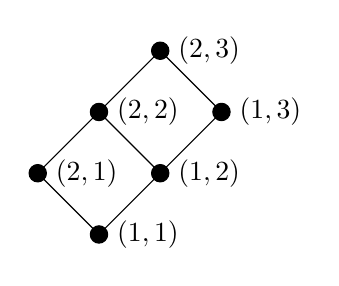
\begin{tikzpicture}[rotate=45,scale=1.1]
%ROWS
\draw (0,0)--(2,0);
\draw (0,1)--(2,1);
%COLUMNS
\draw (0,0)--(0,1);
\draw (1,0)--(1,1);
\draw (2,0)--(2,1);

%POSET NODES
\draw [fill=black] (0,0) circle [radius=0.1cm];
\draw [fill=black] (1,0) circle [radius=0.1cm];
\draw [fill=black] (2,0) circle [radius=0.1cm];

\draw [fill=black] (0,1) circle [radius=0.1cm];
\draw [fill=black] (1,1) circle [radius=0.1cm];
\draw [fill=black] (2,1) circle [radius=0.1cm];

\node at (0.4,-0.4) {$(1,1)$};
\node at (1.4,-0.4) {$(1,2)$};
\node at (2.4,-0.4) {$(1,3)$};

\node at (0.4,0.6) {$(2,1)$};
\node at (1.4,0.6) {$(2,2)$};
\node at (2.4,0.6) {$(2,3)$};
\end{tikzpicture}

\caption{The rectangle $[2] \times [3]$.}
 \label{squareposet}
\end{figure}

\subsection{Rowmotion}

An important object of study in dynamical algebraic combinatorics is a certain dynamical process on order ideals called combinatorial rowmotion.

\begin{Def}
Let $I$ be an order ideal of $P$. \textit{Combinatorial rowmotion} is the map $\rho$ that sends $I$ to the order ideal generated by the minimal elements of $P \setminus I$.
\end{Def}

Cameron and Fon-der-Flaass \cite{cameronfonderflaass} give another description of rowmotion in terms of \textit{combinatorial toggles}. Let $J(P)$ denote the set of order ideals of $P$. For each $p \in P$, we associate a \emph{toggle map} $t_p \colon J(P) \to J(P)$ by
\[t_p(I) = \begin{cases} I \cup \{p\} &\text{ if } p \not\in I \text{ and } I \cup \{p\} \in J(P), \\
I \setminus \{p\} &\text{ if } p \in I \text{ and } I \setminus \{p\} \in J(P), \\
I &\text{ otherwise.} \end{cases}\]
Combinatorial rowmotion can then be defined as the composition of toggles on $P$ in the order of a linear extension $\mathcal L \colon P \to [n]$ (where $n=|P|$) from top to bottom, that is,
\[\rho = t_{\mathcal{L}^{-1}(1)} \circ \dots \circ t_{\mathcal{L}^{-1}(n)}.\]
We note that $t_p \circ t_q = t_q \circ t_p$ if and only if $p$ and $q$ do not form a cover relation. Consequently this description is independent of the choice of linear extension.

In \cite{stanley1}, Stanley gives a bijection (also discovered independently by Thomas) between the order ideals of $R = [r] \times [s]$ and 0/1-sequences with $r$ zeroes and $s$ ones.

\begin{Def}
Let $A$ be an antichain of $R = [r] \times [s]$. The \emph{Stanley--Thomas word} of $A$ is $w(A) = (w_1, \dots, w_{r+s})$, where

\[w_i = \begin{cases} 1 &\text{ if } 1\leq i \leq r \text{ and } A \text{ has an element in row } i, \\ 
1 &\text{ if } r+1 \leq i \leq r+s \text{ and } A \text{ has no element in column } i-r, \\ 
0 &\text{ otherwise.} \end{cases}\]
\end{Def}

Rowmotion performs a cyclic shift of the Stanley--Thomas word \cite{propproby}. Since the map $w$ is a bijection, this gives a simple proof of the following result, originally proved by %Fon-der-Flaass \cite{fonderflaass}.
Brouwer and Schrijver \cite{brouwerschrijver}.

\begin{Th}[\cite{brouwerschrijver}]
The order of $\rho$ on $R=[r] \times [s]$ is $r+s$.
\end{Th}

Note that $r+s$ is one more than the number of distinct ranks of $R$. This is the smallest possible order that rowmotion can have on a graded poset: iteratively applying rowmotion to the empty order ideal simply adds one rank of elements at a time to the order ideal until arriving at the entire poset, which is then mapped back to the empty order ideal.

\subsection{Piecewise-linear rowmotion}

In \cite{stanley2}, Stanley defines two polytopes related to a finite poset.

\begin{Def}
Let $P$ be a finite poset. 

\begin{enumerate}
    \item The \emph{order polytope} $\op \subseteq \mathbb{R}^P$ is the set of all $x \in \mathbb{R}^P$ satisfying the inequalities $0 \leq x_p \leq 1$ for all $p \in P$, and $x_p \leq x_q$ for all $p,q \in P$ satisfying $p \leq q$.
    \item The \emph{chain polytope} $\cp \subseteq \mathbb{R}^P$ is the set of all $x \in \mathbb{R}^P$ satisfying  the inequalities $x_p \geq 0$ for all $p \in P$, and $\sum_{p \in C} x_p \leq 1$ for all (maximal) chains $C \subseteq P$.
\end{enumerate}
\end{Def}
The vertices of $\op$ and $\cp$ are the indicator vectors of the order filters and antichains of $P$, respectively. We may also identify the vertices of $\op$ with the order ideals of $P$ by complementation.

In \cite{stanley2}, Stanley defines a piecewise-linear, continuous, and volume-preserving bijection $\phi \colon \op \to \cp$ called the \emph{transfer map}, defined by
\[\phi(x)_p = x_p - \max\limits_{q \lessdot p} x_q,\]
where we interpret an empty $\max$ as $0$.
The inverse of this map is given by
\[\phi^{-1}(x)_p = \max\limits_{c_1 < c_2 < \dots < c_k = p} \left( \sum\limits_{i=1}^k x_{c_i} \right).\]
The transfer map can be thought of as a piecewise-linear extension of the map that sends an order filter to its minimal elements.

Combinatorial rowmotion permutes order ideals and so can also be thought of as a permutation of the vertices of $\op$. As is the case with the transfer map, there is a natural piecewise-linearization of this bijection described by Einstein and Propp \cite{einsteinpropp1}.

\begin{Def}
The \textit{piecewise-linear toggle} on the order polytope $\op$ corresponding to an element $p \in P$ is the map $t_p\colon \op \to \op$ that changes the $p$th coordinate by
\[x_p \mapsto \min\limits_{q \gtrdot p} x_q + \max\limits_{q \lessdot p} x_q - x_p\]
and fixes all other coordinates, where an empty $\min$ is interpreted as $1$ and an empty $\max$ is interpreted as $0$.
\end{Def}
(We will abuse notation and use the same symbol for combinatorial toggles and piecewise-linear toggles.)
Note that $t_p$ only depends on the coordinates in the neighborhood of $p \in P$ in the Hasse diagram. Consequently for $p,q \in P$, $t_p \circ t_q = t_q \circ t_p$ if and only if neither $p \lessdot q$ nor $p \gtrdot q$ as in the combinatorial realm.

We then define \textit{piecewise-linear rowmotion} $\rho\colon \op \to \op$ using piecewise-linear toggles by
\[\rho = t_{\mathcal{L}^{-1}(1)} \circ \cdots \circ t_{\mathcal{L}^{-1}(|P|)},\]
where $\mathcal{L}$ is any linear extension of $P$.

\subsection{Birational rowmotion}

Piecewise-linear rowmotion can be lifted even further to a birational analogue that uses addition, multiplication, and division in place of $\max$, addition, and subtraction, respectively. This lifting process is called \emph{detropicalization}. (See \cite{einsteinpropp2,einsteinpropp1,noumiyamada} for more detailed discussion.) The functions resulting from detropicalization are generally \emph{subtraction-free} and therefore well-defined on positive labelings of $P$.

As an example, the \emph{birational transfer map} $\phi$ acts on positive labelings $x \in \mathbb R^P_{>0}$ via coordinate functions
\[\phi(x)_p = \frac{x_p}{\sum\limits_{q \lessdot p} x_q}\]
where an empty sum is interpreted as $1$.

Since $\min(a,b) = -\max(-a,-b)$, detropicalizing $\min$ yields the \textit{parallel sum}~$\parallelsum$ defined by
\[a \parallelsum b = \frac{1}{\frac{1}{a} + \frac{1}{b}} = \frac{ab}{a+b}.\]
Parallel sum is associative and commutative. For a finite multiset $S \subseteq \mathbb{R}_{>0}$, we denote the parallel sum of all elements in $S$ by $\sideset{}{^{\parallelsum}} \sum\limits_{s \in S} s$.


\begin{Def}
The \textit{birational toggle} on $\mathbb{R}^{P}_{>0}$ corresponding to an element $p \in P$ is the birational map $t_p\colon \mathbb{R}^{P}_{>0} \to \mathbb{R}^{P}_{>0}$ that changes the $p$th coordinate by
\[x_p \mapsto \left( \sideset{}{^{\parallelsum}} \sum\limits_{q \gtrdot p} x_q \right) \left( \sum\limits_{q \lessdot p} x_q \right) \cdot \frac{1}{x_p}\]
and fixes all other coordinates, where an empty sum or parallel sum is interpreted as $1$.
\end{Def}
(We again abuse notation by using the same notation for birational toggles as piecewise-linear toggles.) Similarly to piecewise-linear rowmotion, we define \textit{birational rowmotion} as
\[\rho = t_{\mathcal{L}^{-1}(1)} \circ \cdots \circ t_{\mathcal{L}^{-1}(|P|)}\]
for any linear extension $\mathcal{L}$ of $P$. From the birational setting, we can obtain the piecewise-linear analogue via a \textit{valuation} or \emph{tropicalization}: see, for instance, \cite{einsteinpropp2,einsteinpropp1}. 

For any poset, one can compute birational rowmotion in terms of the dual transfer map.

\begin{Def}
Let $P$ be a poset and $x \in \mathbb{R}_{>0}^{P}$ be a labeling. The \emph{dual transfer map} is the birational function $\phi^*\colon\mathbb{R}_{>0}^{P} \to \mathbb{R}_{>0}^{P}$ with coordinate functions
\[\phi^*(x)_p = \frac{x_p}{\sum\limits_{q \gtrdot p} x_q}\]
for all $p \in P$, where an empty sum is interpreted as $1$.
\end{Def}

In other words, $\phi^*$ acts on labelings of $P$ in the same way that $\phi$ acts on the associated labeling of the dual of $P$. 

The following lemma is due to Einstein and Propp (see for instance \cite{einsteinpropp2,josephroby2}). We include a short proof for completeness.

\begin{Lemma} \label{lemma:dualtransfer}
Let $P$ be a finite poset. Then for any $x \in \mathbb{R}_{>0}^{P}$ and $p \in P$,
\[ \rho \circ \phi^{-1}(x)_p = \frac{1}{\left(\phi^*\right)^{-1}(x)_p}.\]
\end{Lemma}
\begin{proof}
Let $y = \phi^{-1}(x)$ and $z = (\phi^*)^{-1}(x)$. For any $p \in P$, suppose that $\rho(y)_q = \frac{1}{z_q}$ for all $q > p$. When applying the toggle at $p$ in the computation of $\rho(y)$, the elements at or below $p$ are labeled as in $y$ while those above $p$ are labeled as in $\rho(y)$. Hence by the definition of $t_p$,
\[
    \rho(y)_p =  \left( \sideset{}{^{\parallelsum}} \sum\limits_{q \gtrdot p} \frac{1}{z_q} \right) \left(\sum\limits_{q \lessdot p} y_q \right) \cdot \frac{1}{y_p}  = \frac{1}{\sum\limits_{q \gtrdot p}z_q} \cdot \frac{1}{x_p} = \frac{1}{z_p}.
\]
The result follows easily by induction starting at the top of $P$.
\end{proof}

Computing iterated applications of rowmotion is more difficult. However, one can sometimes prove results about rowmotion using an associated combinatorial construction instead. As mentioned previously, one such example is the Stanley--Thomas word, which lifts to the birational level.

\begin{Def}
Let $R = [r] \times [s]$. The \emph{birational Stanley--Thomas word} $w$ for $x$ is the word of length $r+s$ defined by
\[w_i = \begin{cases} \prod\limits_{j=1}^s x_{ij} &\text{ if } 1\leq i \leq r, \\ \prod\limits_{j=1}^r x_{j,i-r}^{-1} &\text{ if } r+1\leq i \leq r+s.\end{cases}\]
\end{Def}

In \cite{josephroby1} it is shown that $\phi \circ \rho \circ \phi^{-1}$ cyclically shifts the birational Stanley--Thomas word. Though this is not sufficient to show that the order of birational rowmotion on the product of two chains has finite order, it can be used to extend other results (such as instances of homomesy) to the birational level. In Section \ref{section:chainshifting} we  will define a collection of \emph{generalized Stanley--Thomas words}, and in Section \ref{section:greenestheorem} we show that the cyclic rotation of these words uniquely determines rowmotion.

\subsection{Dodgson condensation and the octahedron recurrence} \label{sec:octahedron}

Given a matrix $A=(a_{ij})_{i,j=1}^{n}$, let $A_{ij}^{(k)}$ denote the $k \times k$ submatrix of $A$ formed by the intersection of rows $i$ through $i+k-1$ and columns $j$ through $j+k-1$ whenever $1 \leq i,j \leq n-k+1$. These minors satisfy the following algebraic relation known as the \emph{Desnanot-Jacobi identity}, which forms the basis of a recursive algorithm for computing the determinant of a matrix called \emph{Dodgson condensation}.

\begin{Prop} \label{prop:dodgson}
%desnanot-jacobi identity
For $k \geq 0$,
\[\det(A_{ij}^{(k+1)}) \det(A_{i+1,j+1}^{(k-1)})=\det(A_{ij}^{(k)})\det(A_{i+1,j+1}^{(k)})-\det(A_{i,j+1}^{(k)})\det(A_{i+1,j}^{(k)}).\]
(By convention, we set $\det(A_{ij}^{(0)})=1$ and $\det(A_{ij}^{(-1)})=0$ for all integers $i$ and $j$.)
\end{Prop}

We visualize this relation by placing the values $\det(A_{ij}^{(k)})$ into a three-dimensional array. In all figures containing such an array, we place the entries $\det(A_{ij}^{(k)})$ at height $k$ so that, for $k>1$, $\det(A_{ij}^{(k)})$ lies directly above the center of the submatrix at height $1$ for which it is the determinant. See Figure~\ref{fig:octahedron}.

%Consider the lattice of points $(x,y,z)$ such that $x \equiv y \equiv 0$ mod $2$. If $A \in \mathbb{R}^{r+1 \times s+1}$, define a function $f$ on the subset of the lattice of points (2i, 2j, k) where $0 \leq i \leq r$, $0 \leq j \leq s$, and $0 \leq k \leq \min(r,s)$ by setting
%\begin{align*}
%    f(2i,2j,k) &= \det(A_{ij}^{(k)}).
%\end{align*}
%Visually the point $(x,y,z)$ lies above the center of the submatrix for which $f(x,y,z)$ is the determinant. In Figure~\ref{fig:octahedron}, the top of the pyramid is the determinant of the $2 \times 2$ matrix beneath it.


%Given a matrix $A = (a_{ij})_{i,j = 0}^{r,s}$, we initialize a function on the lattice with $f(2x,2y,0) = 1$ and $f(2i+1, 2j+1, 1) = a_{ij}$. 


%\begin{Def}
%The \emph{Dodgson condensation} is the following recurrence relation: 

%\[f(x-1,y-1,z+1) = \frac{f(x,y,z)f(x-2,y-2,z) - f(x-2,y,z)f(x,y-2,z)}{f(x-1,y-1,z-1)}.\]
%\end{Def}

%Applying Dodgson condensation assigns values to points in a pyramid shape. The value of $f(x,y,z)$ is the solid minor given by the $a_{ij}$ satisfying $\frac{x-z}{2} \leq i \leq \frac{x+z}{2}-1$ and $\frac{y-z}{2} \leq j \leq \frac{y+z}{2}-1$. 



\begin{figure}
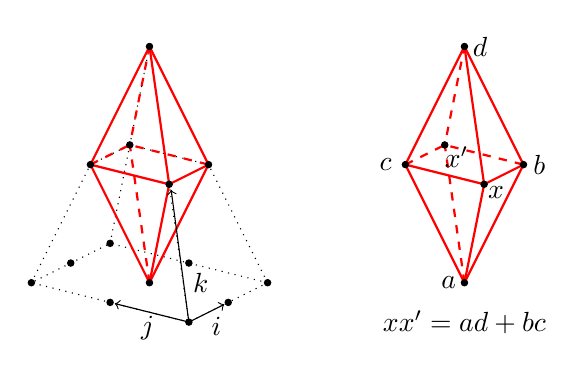
\begin{tikzpicture}[scale = 0.5]

%DOTTED LINES
\draw [dotted] (0,0)--(-4,1)--(-2,2)--(2,1)--cycle;
\draw [dotted] (-0.5,3.5)--(-2.5,4)--(-1.5,4.5)--(0.5,4)--cycle;

\draw [dotted] (0,0)--(-1,7);
\draw [dotted] (-4,1)--(-1,7);
\draw [dotted] (-2,2)--(-1,7);
\draw [dotted] (2,1)--(-1,7);

\draw [red, thick] (-1,1)--(-2.5,4)--(-1,7)--(0.5,4)--cycle;
\draw [red, thick] (-1,1)--(-0.5,3.5)--(-1,7);
\draw [red, thick] (-2.5,4)--(-0.5,3.5)--(0.5,4);

\draw [->] (0,0)--(-1.88,0.47);
\draw [->] (0,0)--(0.9,0.45);
\draw [->] (0,0)--(-0.45,3.36);

\node at (0.7,-0.1) {$i$};
\node at (-1.05,-0.15) {$j$};
\node at (0.3,1) {$k$};
\draw [red, dashed, thick](-1,1)--(-1.5,4.5)--(-1,7);
\draw [red, dashed, thick] (-2.5,4)--(-1.5,4.5)--(0.5,4);


%LAYER 1
\draw [fill=black] (0,0) circle [radius=0.08cm];
\draw [fill=black] (-2,0.5) circle [radius=0.08cm];
\draw [fill=black] (-4,1) circle [radius=0.08cm];

\draw [fill=black] (1,0.5) circle [radius=0.08cm];
\draw [fill=black] (-1,1) circle [radius=0.08cm];
\draw [fill=black] (-3,1.5) circle [radius=0.08cm];

\draw [fill=black] (2,1) circle [radius=0.08cm];
\draw [fill=black] (0,1.5) circle [radius=0.08cm];
\draw [fill=black] (-2,2) circle [radius=0.08cm];

%LAYER 2
\draw [fill=black] (-0.5,3.5) circle [radius=0.08cm];
\draw [fill=black] (-2.5,4) circle [radius=0.08cm];

\draw [fill=black] (0.5,4) circle [radius=0.08cm];
\draw [fill=black] (-1.5,4.5) circle [radius=0.08cm];

%LAYER 3
\draw [fill=black] (-1,7) circle [radius=0.08cm];

\begin{scope}[shift={(9,-1)}]
    \draw [red, thick] (-2,2)--(-3.5,5)--(-2,8)--(-0.5,5)--cycle;
    \draw [red, thick] (-2,2)--(-1.5,4.5)--(-2,8);
    \draw [red, thick] (-3.5,5)--(-1.5,4.5)--(-0.5,5);
    \draw [red, dashed, thick](-2,2)--(-2.5,5.5)--(-2,8);
    \draw [red, dashed, thick] (-3.5,5)--(-2.5,5.5)--(-0.5,5);
    \node at (-1.2,4.3) {$x$};
    \node at (-2.2,5.2) {$x'$};
    \node at (-2.4,2) {$a$};
    \node at (-0.1,5) {$b$};
    \node at (-4,5) {$c$};
    \node at (-1.6,8) {$d$};
    \draw [fill=black] (-2,2) circle [radius=0.08cm];
    \draw [fill=black] (-1.5,4.5) circle [radius=0.08cm];
    \draw [fill=black] (-3.5,5) circle [radius=0.08cm];
    \draw [fill=black] (-0.5,5) circle [radius=0.08cm];
    \draw [fill=black] (-2.5,5.5) circle [radius=0.08cm];
    \draw [fill=black] (-2,8) circle [radius=0.08cm];
    \node at (-2,1){$xx'=ad+bc$};
\end{scope}

\end{tikzpicture}
\caption{The coordinate system we will use for figures depicting three-dimensional arrays $(M_{ij}^{(k)})$. (Note that the $k$ direction does not point vertically but rather along the edge of the pyramid.) 
The octahedron recurrence involves the vertices of translations of the octahedron as shown on the right.
}
\label{fig:octahedron}
\end{figure}


Proposition~\ref{prop:dodgson} then implies that the entries $M_{ij}^{(k)} = \det(A_{ij}^{(k)})$ satisfy the following \emph{octahedron recurrence}:
\[M_{ij}^{(k)}M_{i+1,j+1}^{(k)} = M_{i+1,j+1}^{(k-1)}M_{ij}^{(k+1)}+M_{i+1,j}^{(k)}M_{i,j+1}^{(k)}.\]
The elements in this relation lie at the vertices of an octahedron that is a translation of the one shown in Figure~\ref{fig:octahedron}. By convention, we extend the array $M=(M_{ij}^{(k)})$ to all integers $i$, $j$, and $k$ by setting any undefined values equal to $0$, which does not violate the octahedron recurrence.

%\[f(x,y,z) = \frac{f(x,y,z-1)f(x-2,y-2,z+1)+f(x-2,y,z)f(x,y-2,z)}{f(x-2,y-2,z)}.\]

%\[f(x,y,z) = \frac{f(x-1,y-1,z+1)f(x-1,y-1,z-1) + f(x-2,y,z)f(x,y-2,z)}{f(x-2,y-2,z)}.\]

%For any octahedron shape, if we know 5 of the values of $f$, then we can compute the 6th by solving for it in the Dodgson condensation formula.  Solving for $f(x,y,z)$ yields
%\[f(x,y,z) = \frac{f(x-1,y-1,z+1)f(x-1,y-1,z-1) + f(x-2,y,z)f(x,y-2,z)}{f(x-2,y-2,z)}.\]
%which is called the \emph{octahedron recurrence}. In TODO:CITE HOPKINS, Hopkins used the octahedron recurrence to prove a special case of the rowmotion formula. 

We now demonstrate the known relationship between toggles and the octahedron recurrence appearing in  \cite{grinbergroby2}. A visualization of this lemma is shown in Figure~\ref{fig:toggle}. If part of the rectangle poset is labeled via the quotients $z_{ij}^{(k)}$ as shown, then Lemma~\ref{lemma:arraytoggle} shows that a toggle at $(i,j)$ transforms $z_{ij}^{(k-1)}$ to $z_{ij}^{(k)}$.

\begin{Lemma}\label{lemma:arraytoggle}
Suppose $M = (M_{ij}^{(k)})$ is an array of indeterminates satisfying the octahedron recurrence, and let $z_{ij}^{(k)} = \frac{M_{k+2,i+k+1}^{(j-1)}}{M_{k+1,i+k+1}^{(j)}}$.
Then as rational functions in the entries of $M$, \[z_{ij}^{(k)} = \frac{(z_{i,j-1}^{(k)}+z_{i-1,j}^{(k)})(z_{i+1,j}^{(k-1)}\parallelsum z_{i,j+1}^{(k-1)})}{z_{ij}^{(k-1)}}.\]



%Let $R = [0,r] \times [0,s]$ and let $z \in \mathbb{R}_{>0}^{R}$ be a positive labeling of $R$. 


%If a function $f$ of the form described above satisfies the octahedron recurrence and if 
%\begin{align*}
%    &z_{i+1,j} = \frac{f(2,2i+4,j)}{f(0,2i+4,j+1)} & &z_{i,j+1} = \frac{f(2,2i+2,j+1)}{f(0,2i+2,j+2)} \\
%    & &z_{ij} = \frac{f(2,2i+2,j)}{f(0,2i+2,j+1)} \\
%    &z_{i,j-1} = \frac{f(4,2i+4,j-1)}{f(2,2i+4,j)}& &z_{i-1,j} = \frac{f(4,2i+2,j)}{f(2,2i+2,j+1)} \\
%\end{align*}
%\noindent then,
%\[t_{ij}(z)_{ij} = \frac{f(4,2i+4,j)}{f(2,2i+4,j+1)}.\]
\end{Lemma}




\begin{figure}
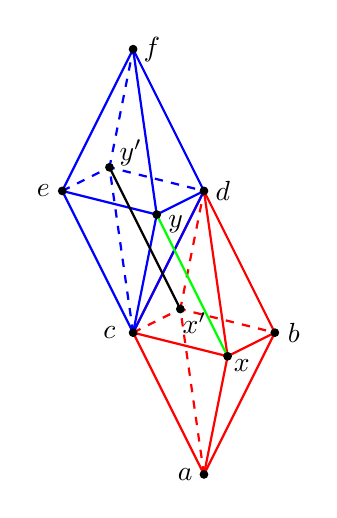
\begin{tikzpicture}[scale = 0.6]

\draw [red, thick] (-2,2)--(-3.5,5)--(-2,8)--(-0.5,5)--cycle;
\draw [red, thick] (-2,2)--(-1.5,4.5)--(-2,8);
\draw [red, thick] (-3.5,5)--(-1.5,4.5)--(-0.5,5);
\draw [red, dashed, thick](-2,2)--(-2.5,5.5)--(-2,8);
\draw [red, dashed, thick] (-3.5,5)--(-2.5,5.5)--(-0.5,5);

\draw [blue, thick] (-3.5,5)--(-5,8)--(-3.5,11)--(-2,8)--cycle;
\draw [blue, thick] (-3.5,5)--(-3,7.5)--(-3.5,11);
\draw [blue, thick] (-5,8)--(-3,7.5)--(-2,8);
\draw [blue, dashed, thick](-3.5,5)--(-4,8.5)--(-3.5,11);
\draw [blue, dashed, thick] (-5,8)--(-4,8.5)--(-2,8);

\draw [green, thick] (-1.5,4.5)--(-3,7.5);
\draw [black, thick] (-2.5,5.5)--(-4,8.5);

%LAYER 1
\draw [fill=black] (-2,2) circle [radius=0.08cm];

%LAYER 2
\draw [fill=black] (-1.5,4.5) circle [radius=0.08cm];
\draw [fill=black] (-3.5,5) circle [radius=0.08cm];

\draw [fill=black] (-0.5,5) circle [radius=0.08cm];
\draw [fill=black] (-2.5,5.5) circle [radius=0.08cm];

%LAYER 3
\draw [fill=black] (-3,7.5) circle [radius=0.08cm];
\draw [fill=black] (-5,8) circle [radius=0.08cm];

\draw [fill=black] (-2,8) circle [radius=0.08cm];
\draw [fill=black] (-4,8.5) circle [radius=0.08cm];

%LAYER 4
\draw [fill=black] (-3.5,11) circle [radius=0.08cm];

\node at (-1.2,4.3) {$x$};
\node at (-2.2,5.2) {$x'$};

\node at (-2.6,7.3) {$y$};
\node at (-3.55,8.8) {$y'$};

\node at (-2.4,2) {$a$};
\node at (-0.1,5) {$b$};
\node at (-4,5) {$c$};
\node at (-1.6,8) {$d$};
\node at (-5.4,8) {$e$};
\node at (-3.1,11) {$f$};

\end{tikzpicture}
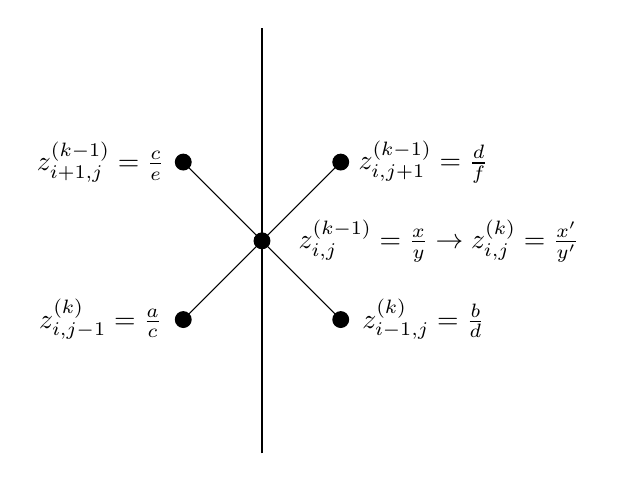
\begin{tikzpicture}
\transparent{0.0}
\draw (0,-2.7)--(0,2.7);
\transparent{1.0}

\draw (-1,-1)--(1,1);
\draw (-1,1)--(1,-1);

\draw [fill=black] (-1,-1) circle [radius=0.1cm];
\draw [fill=black] (1,-1) circle [radius=0.1cm];

\draw [fill=black] (0,0) circle [radius=0.1cm];

\draw [fill=black] (-1,1) circle [radius=0.1cm];
\draw [fill=black] (1,1) circle [radius=0.1cm];

\node at (-2.05,-1) {$z_{i,j-1}^{(k)} = \frac{a}{c}$};
\node at (2.05,-1) {$z_{i-1,j}^{(k)} = \frac{b}{d}$};

\node at (2.25,0) {$z_{i,j}^{(k-1)} = \frac{x}{y}\to z_{i,j}^{(k)} = \frac{x'}{y'}$};

\node at (-2.05,1) {$z_{i+1,j}^{(k-1)} = \frac{c}{e}$};
\node at (2.05,1) {$z_{i,j+1}^{(k-1)} = \frac{d}{f}$};
\end{tikzpicture}
\caption{The relationship between the octahedron recurrence and birational toggles as described in Lemma~\ref{lemma:arraytoggle}. Two labelings of the poset by quotients of entries in the octahedron recurrence are related by a birational toggle at the central element.}
\label{fig:toggle}
\end{figure}

\begin{proof} For ease of notation, we relabel the relevant part of the array as in Figure~\ref{fig:toggle}. (For instance, $x = M_{k+1,i+k}^{(j-1)}$ and $y = M_{k,i+k}^{(j)}$, so $z_{ij}^{(k-1)} = \frac{x}{y}$.) Applying the octahedron recurrence to the two octahedra shown and dividing gives
%We will show that if the array satisfies the octahedron recurrence, then $t_{ij}(z)_{ij} = \frac{x'}{y'}$. Indeed: %Thus applying rowmotion gives the labeling stored in the edges after shifting by the vector (2,2,0).
%Let $z \in \mathbb{R}_{>0}^{|R|}$. 
%Given a portion of the array as shown in Figure~\ref{fig:toggle}, consider a point $z \in \mathbb{R}_{>0}^{|R|}$ labeled by:
%\begin{align*}
%    z_{i+1,j} &= \tfrac{c}{e} \\
%    z_{i,j+1} &= \tfrac{d}{f} \\
%    z_{i,j} &= \tfrac{x}{y} \\
%    \rho^{-1}(z)_{i,j-1} = \tfrac{a}{c} \\
%    \rho^{-1}(z)_{i-1,j} = \tfrac{b}{d}
%    z_{i,j-1} &= \tfrac{a}{c} \\
%    z_{i-1,j} &= \tfrac{b}{d}
%\end{align*}
\begin{align*}
    \frac{xx'}{yy'} &= \frac{ad+bc}{cf+de} 
%    &= \frac{cd\left( \frac{a}{c} + \frac{b}{d} \right)}{cd\left(\frac{f}{d} + \frac{e}{c}\right)} \\
= \frac{\frac{a}{c} + \frac{b}{d}}{\frac{f}{d} + \frac{e}{c}}
%    &= \frac{ \frac{a}{c} + \frac{b}{d} }{\frac{1}{ \left(\frac{d}{f}\right) } + \frac{1}{ \left(\frac{c}{e}\right) } } \\
    = \left( \frac{a}{c} + \frac{b}{d} \right) \left(\frac{d}{f} \parallelsum  \frac{c}{e} \right).  
\end{align*}
Solving for $\frac{x'}{y'}$ yields the desired identity
%\[\frac{x'}{y'}=  \left( \frac{a}{c} + \frac{b}{d} \right) \left(\frac{d}{f} \parallelsum  \frac{c}{e} \right)\left(\frac{y}{x} \right) =  \left( z_{i,j-1} + z_{i-1,j} \right) \left(z_{i,j+1} \parallelsum  z_{i+1,j} \right)\frac{1}{z_{i,j}} = t_{ij}(z)_{ij}\]
\[\frac{x'}{y'}=  \frac{\left( \frac{a}{c} + \frac{b}{d} \right) \left(\frac{c}{e} \parallelsum  \frac{d}{f} \right)}{\frac xy}.\qedhere\]
\end{proof}

\begin{Rem} \label{rem:arraytoggle}
In most cases when we apply Lemma~\ref{lemma:arraytoggle}, all quantities will specialize to well-defined values. There are two exceptions: if we set $e = M_{k,i+k+1}^{(j)} = 0$ (which would make $\frac ce = z_{i+1,j}^{(k-1)}$ undefined), then in the proof we instead have
\begin{align*}
    \frac{xx'}{yy'} &= \frac{ad+bc}{cf} 
%    &= \frac{cd\left( \frac{a}{c} + \frac{b}{d} \right)}{cd\left(\frac{f}{d} + \frac{e}{c}\right)} \\
= \frac{\frac{a}{c} + \frac{b}{d}}{\frac{f}{d}}
%    &= \frac{ \frac{a}{c} + \frac{b}{d} }{\frac{1}{ \left(\frac{d}{f}\right) } + \frac{1}{ \left(\frac{c}{e}\right) } } \\
    = \left( \frac{a}{c} + \frac{b}{d} \right) \left(\frac{d}{f} \right),  
\end{align*}
which yields the same result as Lemma~\ref{lemma:arraytoggle} but with the undefined term $z_{i+1,j}^{(k-1)}$ removed from the parallel sum.
%\[z_{ij}^{(k+1)} = \frac{(z_{i,j-1}^{(k+1)}+z_{i-1,j}^{(k+1)})(z_{i,j+1}^{(k)})}{z_{ij}^{(k)}}.\]
%Note that if in the proof above we set $e = M_{k,i+k+2}^{(j+1)} = 0$ (which would make $\frac ce = z_{i+1,j}^{(k)}$ undefined), we instead arrive at 
%\[z_{ij}^{(k+1)} = \frac{(z_{i,j-1}^{(k+1)}+z_{i-1,j}^{(k+1)})(z_{i,j+1}^{(k)})}{z_{ij}^{(k)}}.\]
A similar result holds if we instead set $f = M_{k,i+k}^{(j+1)}=0$ (which would make $\frac{d}{f} = z_{i,j+1}^{(k-1)}$ undefined).
\end{Rem}


Lemma~\ref{lemma:arraytoggle} suggests that toggling/rowmotion should be thought of as translation with respect to the octahedron recurrence. In the next section, we will see how this relationship can be used to prove the iterated birational rowmotion formula for rectangles.

\section{Birational rowmotion in the rectangle poset} \label{section:rowmotiononrectangles}

In this section, we will use the relationship between the octahedron recurrence and toggles to prove a formula for any power of birational rowmotion on a rectangle similar to one given by Musiker--Roby \cite{musikerroby}. This formula will be described in terms of nonintersecting paths inside a certain graph $\mathcal G_R$. We will begin by proving a lemma that relates nonintersecting paths in $\mathcal G_R$ to nonintersecting paths in $R$.

\subsection{Nonintersecting paths} \label{sec:paths}
Let $R=[r] \times [s]$, and let the element $(i,j)$ have weight $x_{ij}$. For $1 \leq k \leq s$, define $\mathcal P^{(k)}_R$ to be the set of all collections $\mathcal L$ of $k$ nonintersecting (i.e. vertex disjoint) paths traveling up along the edges of the Hasse diagram of $R$, starting at $\{(1,1), (1,2), \dots, (1,k)\}$ and ending at $\{(r,s-k+1),\dots,(r,s)\}$. The \emph{weight} $w(\mathcal L)$ is the product of the weights of the elements in the paths of $\mathcal L$. We will write $w_R^{(k)} = w_R^{(k)}(x)$ for the sum of the weights of all collections of paths in $\mathcal P^{(k)}_R$.  We also write $w_R = w_R^{(s)}$ for the product of all weights in $R$.   Similarly, if $I$ is any interval in $R$, then we define $\mathcal P_I^{(k)}$, $w_I^{(k)}(x)$, and $w_I$ in an analogous manner.

Note that while the definition of $\mathcal P_R^{(k)}$ is asymmetric in $r$ and $s$, if $k \leq \min\{r,s\}$, then the paths in any $\mathcal L \in \mathcal P_R^{(k)}$ must pass through all $k$ elements at rank $k+1$ as well as those at rank $r+s-k+1$. Thus in this case $w_R^{(k)}$ will remain unchanged if we transpose $R$. %(In addition, it is simple to verify that $w_R^{(k)} = w_R$ if $k \geq \min\{r,s\}$.)
We will generally assume that $k \leq \min\{r,s\}$ when considering $\mathcal P_R^{(k)}$.

Define $\mathcal{G}_R$ to be the graph with vertex set $[r+1] \times [s]$, directed edges from $(i,j)$ to $(i+1,j)$ of weight $x_{ij}^{-1}$, and directed edges from $(i,j)$ to $(i+1,j-1)$ of weight 1. (The vertices of $R$ are in bijection with the edges of $\mathcal{G}_R$ whose weights are not $1$.)
As an example, Figure~\ref{fig:poset_and_graph} shows $R = [2] \times [3]$ and the corresponding graph $\mathcal G_R$.

We label the vertices on the boundary of $\mathcal G_R$ as follows: for $1 \leq i \leq r$ and $1 \leq j \leq s$, define
\[P_j = (1, j), \quad P_{s+i} = (i+1, s), \quad Q_i = (i,1), \quad Q_{r+j} = (r+1, j).\]
We then define $\mathcal S^{(k)}_{ij}$ to be the set of all collections $\mathcal L'$ of $k$ nonintersecting paths starting from $\{P_i, \dots, P_{i+k-1}\}$ and ending at $\{Q_j, \dots, Q_{j+k-1}\}$. The \emph{weight} $w(\mathcal L')$ of $\mathcal L'$ is the product of the weights of the edges in the paths of $\mathcal L'$. Let $W_{ij}^{(k)} = W_{ij}^{(k)}(x)$ be the total weight of all $\mathcal L' \in \mathcal S^{(k)}_{ij}$. (By convention, $W_{ij}^{(0)} = 1$ and $W_{ij}^{(k)} = 0$ when $k < 0$.)

%%%%%%%%%%%%%%%%%%%%%%%%%%%%%

\begin{figure}
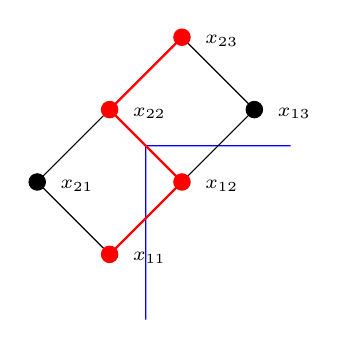
\begin{tikzpicture}[scale = 1.3, rotate = 135]
\transparent{0.0};
\draw [blue] (-0.7,0.2)--(0.5,-1);
\draw [blue] (0.5,-1)--(-0.5,-2);
\transparent{1.0};

%EDGES
\draw (0,0)--(1,0);
\draw [red,thick] (0,-1)--(1,-1);
\draw (0,-2)--(1,-2);

\draw [thick, red] (0,0)--(0,-1);
\draw (0,-1)--(0,-2);
\draw (1,0)--(1,-1);
\draw [thick, red] (1,-1)--(1,-2);

%NODES
\draw [red, fill=red] (0,0) circle [radius=0.08cm];
\draw [fill=black] (1,0) circle [radius=0.08cm];

\draw [red, fill=red] (0,-1) circle [radius=0.08cm];
\draw [red, fill=red] (1,-1) circle [radius=0.08cm];

\draw [fill=black] (0,-2) circle [radius=0.08cm];
\draw [red, fill=red] (1,-2) circle [radius=0.08cm];

\begin{scriptsize}
\node at (-0.3,-0.25) {$x_{11}$};
\node at (-0.3,-1.25) {$x_{12}$};
\node at (-0.3,-2.25) {$x_{13}$};

\node at (0.7,-0.25) {$x_{21}$};
\node at (0.7,-1.25) {$x_{22}$};
\node at (0.7,-2.25) {$x_{23}$};
\end{scriptsize}

\end{tikzpicture}
% \begin{tikzpicture}[scale = 1.3]
% \transparent{0.0}
% \draw [blue] (2,0)--(2,-1.7);
% \draw [blue] (1.6,0)--(3.7,0);
% \transparent{1.0};
% \draw (2,0.1)--(3,0.1)--(3,0.2)--(3.5,0)--(3,-0.2)--(3,-0.1)--(2,-0.1)--cycle;
% \end{tikzpicture}
\qquad
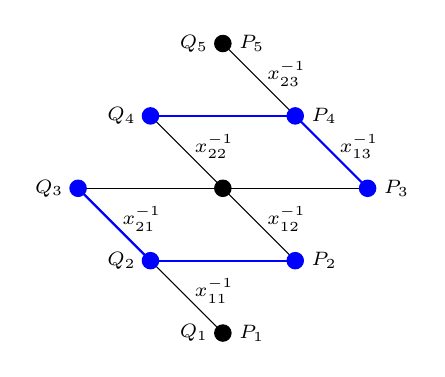
\begin{tikzpicture}[scale = 1.3, rotate = 135]
%EDGES
\draw (0,0)--(1,0);
\draw [blue, thick] (1,0)--(2,0);
\draw (0,-1)--(2,-1);
\draw [blue, thick] (0,-2)--(1,-2);
\draw (1,-2)--(2,-2);

\draw [blue, thick] (0,-1)--(1,0);
\draw (0,-2)--(2,0);
\draw [blue, thick] (1,-2)--(2,-1);

%NODES
\draw [fill=black] (0,0) circle [radius=0.08cm];
\draw [blue, fill=blue] (1,0) circle [radius=0.08cm];
\draw [blue, fill=blue] (2,0) circle [radius=0.08cm];

\draw [blue, fill=blue] (0,-1) circle [radius=0.08cm];
\draw [fill=black] (1,-1) circle [radius=0.08cm];
\draw [blue, fill=blue] (2,-1) circle [radius=0.08cm];

\draw [blue, fill=blue] (0,-2) circle [radius=0.08cm];
\draw [blue, fill=blue] (1,-2) circle [radius=0.08cm];
\draw [fill=black] (2,-2) circle [radius=0.08cm];

\begin{scriptsize}
\node at (-0.2,-0.2) {$P_1$};
\node at (-0.2,-1.2) {$P_2$};
\node at (-0.2,-2.2) {$P_3$};
\node at (0.8,-2.2) {$P_4$};
\node at (1.8,-2.2) {$P_5$};

\node at (0.2,0.2) {$Q_1$};
\node at (1.2,0.2) {$Q_2$};
\node at (2.2,0.2) {$Q_3$};
\node at (2.2,-0.8) {$Q_4$};
\node at (2.2,-1.8) {$Q_5$};

\node at (0.35,-0.23) {$x_{11}^{-1}$};
\node at (1.35,-0.23) {$x_{21}^{-1}$};

\node at (0.35,-1.23) {$x_{12}^{-1}$};
\node at (1.35,-1.23) {$x_{22}^{-1}$};

\node at (0.35,-2.23) {$x_{13}^{-1}$};
\node at (1.35,-2.23) {$x_{23}^{-1}$};
\end{scriptsize}
\end{tikzpicture}
\caption{The poset $R$ and graph $\mathcal G_R$ for $r=2$ and $s=3$. Edges are directed up and to the left in $\mathcal{G}_{R}$, and unlabeled edges have weight $1$. The highlighted paths correspond via the bijection in Lemma~\ref{pathsinideal}.}
\label{fig:poset_and_graph}
\end{figure}

The following result relates paths in $R$ to paths in $\mathcal{G}_R$.

\begin{Lemma} \label{lemma:gr}
%There exists a bijection that sends each $\mathcal L \in \mathcal P_R^{(k)}$ to $\mathcal L' \in \mathcal S_{k,r+1}^{(s-k+1)}$ such that $w(\mathcal L') = \frac{w(\mathcal L)}{w(R)}$.
There exists a bijection from $\mathcal P_R^{(k)}$ to $\mathcal S_{k+1,r+1}^{(s-k)}$ that divides weight by $w_R$.
%collections $\mathcal L$ of nonintersecting lattice paths in $R$ from $A = \{(0,0),\dots ,(0,k)\}$ to $B = \{(r,s-k),\dots,(r,s)\}$ and collections $\mathcal L'$ of nonintersecting paths in $\mathcal{G}_R$ from $A' = \{P_{k+1},\dots, P_s\}$ to $B' = \{Q_{r+1},\dots,Q_{r+s-k}\}$. Under this bijection, the weight of $\mathcal L$ corresponds to the inverse weight of $\mathcal L'$.
\end{Lemma}

\begin{figure}
    \centering
    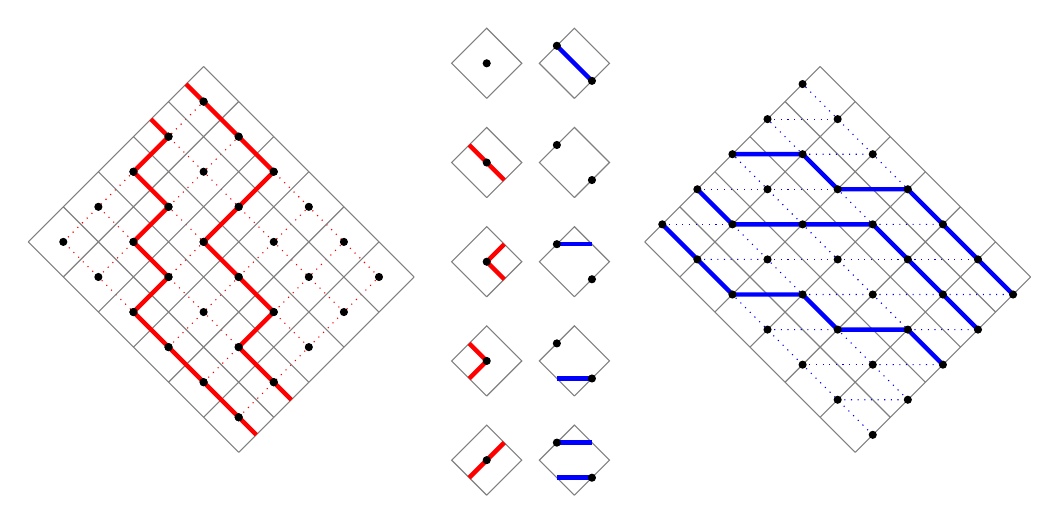
\begin{tikzpicture}[scale=0.9]
        \tikzstyle{w}=[circle, draw, fill=black, inner sep=0pt, minimum width=2.5pt]
        \begin{scope}[rotate=45,scale=.7]
        \draw[dotted,red] (0,0) grid (4,5);
        \draw[gray,thin,shift={(-.5,-.5)}] (0,0) grid (5,6);
        \draw[red, ultra thick] (0,-.5)--(0,3)--(1,3)--(1,4)--(2,4)--(2,5)--(3,5)--(3,5.5);
        \draw[red, ultra thick] (1,-.5)--(1,1)--(2,1)--(2,3)--(4,3)--(4,5.5);
        \foreach \x in {0,...,4}
            \foreach \y in {0,...,5}
                \node(\x\y)[w] at (\x,\y){};
        \foreach \x/\y in {0/0,0/1,0/2,0/3,1/3,1/4,2/4,2/5,3/5,1/0,1/1,2/1,2/2,2/3,3/3,4/3,4/4,4/5}
            \node[w] at (\x,\y){};
        \end{scope}
        
        \begin{scope}[shift={(3.5,4.5)},scale=.495]
        \draw[gray, thin] (0,0)--(1,1)--(0,2)--(-1,1)--(0,0);
        \node[w] at (0,1){};
        \draw[gray, thin] (2.5,0)--(3.5,1)--(2.5,2)--(1.5,1)--(2.5,0);
        \draw[blue, ultra thick] (3,.5)--(2,1.5);
        \node[w] at (3,.5){};
        \node[w] at (2,1.5){};
        \end{scope}
        \begin{scope}[shift={(3.5,3.1)},scale=.495]
        \draw[gray, thin] (0,0)--(1,1)--(0,2)--(-1,1)--(0,0);
        \draw[red, ultra thick] (.5,.5)--(-.5,1.5);
        \node[w] at (0,1){};
        \draw[gray, thin] (2.5,0)--(3.5,1)--(2.5,2)--(1.5,1)--(2.5,0);
        %\draw[blue, ultra thick] (3,.5)--(2,1.5);
        \node[w] at (3,.5){};
        \node[w] at (2,1.5){};
        \end{scope}
        \begin{scope}[shift={(3.5,1.7)},scale=.495]
        \draw[gray, thin] (0,0)--(1,1)--(0,2)--(-1,1)--(0,0);
        \draw[red, ultra thick] (.5,.5)--(0,1)--(.5,1.5);
        \node[w] at (0,1){};
        \draw[gray, thin] (2.5,0)--(3.5,1)--(2.5,2)--(1.5,1)--(2.5,0);
        \draw[blue, ultra thick] (3,1.5)--(2,1.5);
        \node[w] at (3,.5){};
        \node[w] at (2,1.5){};
        \end{scope}
        \begin{scope}[shift={(3.5,0.3)},scale=.495]
        \draw[gray, thin] (0,0)--(1,1)--(0,2)--(-1,1)--(0,0);
        \draw[red, ultra thick] (-.5,.5)--(0,1)--(-.5,1.5);
        \node[w] at (0,1){};
        \draw[gray, thin] (2.5,0)--(3.5,1)--(2.5,2)--(1.5,1)--(2.5,0);
        \draw[blue, ultra thick] (3,.5)--(2,.5);
        \node[w] at (3,.5){};
        \node[w] at (2,1.5){};
        \end{scope}
        \begin{scope}[shift={(3.5,-1.1)},scale=.495]
        \draw[gray, thin] (0,0)--(1,1)--(0,2)--(-1,1)--(0,0);
        \draw[red, ultra thick] (-.5,.5)--(0,1)--(.5,1.5);
        \node[w] at (0,1){};
        \draw[gray, thin] (2.5,0)--(3.5,1)--(2.5,2)--(1.5,1)--(2.5,0);
        \draw[blue, ultra thick] (3,1.5)--(2,1.5) (3,.5)--(2,.5);
        \node[w] at (3,.5){};
        \node[w] at (2,1.5){};
        \end{scope}
        
        \begin{scope}[shift={(8.7,0)},rotate=45,scale=.7]
        \draw[gray,thin,shift={(-.5,-.5)}] (0,0) grid (5,6);
        \foreach \x in {0,...,4}
            \draw[dotted,blue] (\x,-.5)--(\x,5.5);
        \foreach \x in {0,...,3}
            \foreach \y in {1,...,6}
                \draw[dotted,blue] (\x,\y-.5)--(\x+1,\y-1.5);
        \draw[blue, ultra thick] (2,-.5)--(2,.5)--(1,1.5)--(1,2.5)--(0,3.5)--(0,5.5);
        \draw[blue, ultra thick] (3,-.5)--(3,2.5)--(1,4.5)--(1,5.5);
        \draw[blue, ultra thick] (4,-.5)--(4,2.5)--(3,3.5)--(3,4.5)--(2,5.5);
        \foreach \x in {0,...,4}
            \foreach \y in {0,...,6}
                \node(\x\y)[w] at (\x,\y-.5){};
        \end{scope}
    \end{tikzpicture}
    \caption{Bijection between $\mathcal P_R^{(k)}$ and $\mathcal S_{k+1,r+1}^{(s-k)}$ as in Lemma~\ref{lemma:gr}. Tiles on the left are replaced with the corresponding tiles on the right.}
    \label{fig:5-vertex}
\end{figure}

\begin{proof}
In the drawing of $\mathcal L \in \mathcal P^{(k)}_R$, extend the start and end of each path by a half-edge from northwest to southeast. Such a drawing can be built by piecing together square tiles centered at each vertex showing the five ways in which the paths can pass through that vertex in such a way that the tiles match along sides---see Figure~\ref{fig:5-vertex}. We can replace each tile with a new tile containing edges/half-edges parallel to the edges of $\mathcal G_R$ in a way that preserves the exits along the southwest and northeast sides but inverts the exits along the southeast and northwest sides as shown in Figure~\ref{fig:5-vertex}. Placing vertices on the southeast and northwest edges of these new tiles, the resulting drawing will then depict a collection of paths $\mathcal L'$ in $\mathcal G_R$ that forms an element of $\mathcal S_{k+1,r+1}^{(s-k)}$. (This bijection also has the following alternate description: when the two drawings are overlaid, each of the $k$ horizontal steps in the $i$th path in $\mathcal L'$ crosses the $i$th northeast step in one of the $k$ paths in $\mathcal L$.)

The weighted edges in $\mathcal L'$ correspond to elements of $R$ not lying in any path of $\mathcal L$. Thus $w(\mathcal L')$ is the inverse of the weight of the complement of $\mathcal L$ in $R$, which is exactly $\frac{w(\mathcal L)}{w_R}$.
\end{proof}


% \begin{proof}
% We overlay $R$ and $\mathcal G_R$ so that $(i,j) \in R$ coincides with $(i,j) \in \mathcal G_R$. Let $\mathcal L = \{L_1, \dots, L_k\}$ be a collection of nonintersecting paths from $A = \{(0,0),\dots ,(0,k-1)\}$ to $B = \{(r,s-k+1),\dots,(r,s)\}$ in $R$. We construct paths $\mathcal L' = \{L_{k}', \dots, L_s'\}$ starting at the elements of $A' = \{P_{k},\dots, P_s\}$ in $\mathcal G_R$ as follows: starting each path $L_i'$ at $P_i$, repeatedly extend each path to the northwest if its current endpoint does not lie in any path of $\mathcal L$, otherwise extend it to the west. In other words, in the overlaid diagrams, each $L_i'$ contains a horizontal step immediately after crossing some $L_j$ (i.e. touching the endpoint of a northeast step in $\mathcal L$). See Figure~\ref{fig:overlay}. Note that a path $L_i'$ cannot cross $L_j$ at the endpoint of a northwest step in $L_j$ since the first time this happens would require both a northwest and northeast step starting at the same point in $\mathcal L$.

% After a fixed number of steps, $L_p'$ must cross at least as many paths in $\mathcal L$ as $L_q'$ if $p < q$. Therefore $L_p'$ will have taken at least as many horizontal steps, so the paths in $\mathcal L'$ do not intersect. Since the paths in $\mathcal L$ must together contain all elements in the top $k$ ranks of $R$, no path in $\mathcal L'$ can contain any point in the top $k-1$ ranks of $R$, so each path in $\mathcal L'$ must cross each path in $\mathcal L$. It follows that $\mathcal L'$ is a collection of nonintersecting paths starting from $A'$ and ending at $B' = \{Q_{r+1},\dots,Q_{r+s-k+1}\}$.

% The inverse map is constructed similarly: given $\mathcal L'$, start paths at the elements of $A$ and step to the northwest unless the new point lies in one of the $L_i'$ (i.e. at the end of a horizontal step in $L_i'$), in which case step to the northeast instead. A similar argument as above shows that this defines a collection of nonintersecting paths $\mathcal L$ from $A$ to $B$ in $R$. These maps are inverses because $\mathcal L'$ and $\mathcal L$ are determined by their horizontal and northeast steps, respectively, which are constructed to be incident in both cases.

% By construction, no northwest step in $\mathcal L'$ can start at the beginning or end of any northwest step in $\mathcal L$. Thus the inverse weight of any edge used in $\mathcal L'$ is not the weight of any vertex used in $\mathcal L$. A simple counting argument then shows that every variable $x_{ij}$ appears in exactly one $w(\mathcal L)$ and $w(\mathcal L')^{-1}$, which proves the claim.
% \end{proof}



% \begin{proof}
% We overlay $R$ and $\mathcal{G}_R$ such that $(i,j) \in R$ coincides with $(i,j) \in \mathcal{G}_R$. Let $(V,E)$ be the sets of vertices and edges in a set of nonintersecting lattice paths in $R$. We define $V'$ to be the set of vertices $(i,j)$ in $\mathcal{G}_R$ such that there is no edge $(i-1,j) \to (i,j) \in E$. We claim that there exists a unique set of edges $E'$ in $\mathcal{G}_R$ such that $(V',E')$ forms a collection of nonintersecting paths. The uniqueness is clear, so we need only prove existence.



% Let $E'$ be the set of edges in $\mathcal{G}_R$ starting at $(i,j) \in V'$ of the form $(i,j) \to (i+1,j-1)$ if $(i,j-1) \to (i,j) \in E$ and $(i,j) \to (i+1,j)$ otherwise. It follows that from each $(i,j)$ with $i \leq r$, there is exactly one edge in $E'$ exiting $(i,j)$. 

% \begin{figure}[h]
%     \centering
% \begin{tikzpicture}
% \draw [very thick, red] (0,0)--(1,1);
% \draw [very thick, blue] (1,1)--(-1,1);

% \draw [fill=black] (-1,1) circle [radius=0.1cm];
% \draw [fill=black] (1,1) circle [radius=0.1cm];
% \draw [fill=black] (0,0) circle [radius=0.1cm];
% \draw [fill=black] (0,2) circle [radius=0.1cm];

% \begin{scriptsize}
% \node at (1,1.3) {$(i,j)$};
% \node at (-1,1.3) {$(i+1,j-1)$};
% \node at (-0.8,0) {$(i,j-1)$};
% \end{scriptsize}




% \foreach \x in {4}{
% \draw [xshift = \x cm, very thick, blue] (1,1)--(0,2);

% \draw [xshift = \x cm, fill=black] (-1,1) circle [radius=0.1cm];
% \draw [xshift = \x cm, fill=black] (1,1) circle [radius=0.1cm];
% \draw [xshift = \x cm, fill=black] (0,2) circle [radius=0.1cm];
% \draw [xshift = \x cm, fill=black] (0,0) circle [radius=0.1cm];

% \begin{scriptsize}
% \node [xshift = \x cm] at (-1,1.3) {$(i+1,j-1)$};
% \node [xshift = \x cm] at (1.1,2) {$(i+1,j)$};
% \node [xshift = \x cm] at (1,0.7) {$(i,j)$};
% \end{scriptsize}
% }
% \end{tikzpicture}
%     \caption{The blue edges in $E'$ are determined by the red edges of $E$}
%     \label{fig:my_label}
% \end{figure}

% If $(i,j) \to (i+1,j-1) \in E'$, then $(i,j-1) \to (i,j) \in E$ and so we cannot have $(i,j-1) \to (i+1,j-1) \in E'$ (because the lattice paths are not intersecting). If $(i,j) \to (i+1,j) \in E'$, then $(i,j-1) \to (i,j) \not\in E$. If $(i+1,j) \not\in V'$, then there must be an edge $(i,j) \to (i+1,j) \in E$. This edge must be preceded by an edge of the form $(i-1,j) \to (i,j) \in E$, so $(i,j) \not\in V'$, a contradiction. Hence the edges of $E'$ end in $V'$.

% If we have both $(i-1,j) \to (i,j) \in E'$ and $(i-1,j+1) \to (i,j) \in E'$, then we have $(i-1,j) \to (i-1,j+1) \in E$ and $(i-1,j-1) \to (i-1,j) \not\in E$. Consequently $(i-2,j) \to (i-1,j) \in E$, and so $(i-1,j) \not \in V'$, a contradiction.

% If we have neither of these edges in $E'$, then there are $r+s-k$ points at which paths can end and more than $r+s-k$ paths. By the pigeonhole principle two paths must both enter the same point, which we said was not possible. Hence the pair $(V',E')$ forms a set of nonintersecting lattice paths in $\mathcal{G}_R$. The inverse is similar.
% \begin{figure}
% \begin{tikzpicture}[scale = 1]
% \draw [very thick, blue] (0,0)--(-1,1);
% \draw [very thick, blue] (0,0)--(-2,0);

% \draw [fill=black] (0,0) circle [radius=0.1cm];
% \draw [fill=black] (-1,1) circle [radius=0.1cm];
% \draw [fill=black] (-2,0) circle [radius=0.1cm];

% \begin{small}
% \node at (0.55,0) {$(i,j)$};
% \node at (-1.9,1) {$(i+1,j)$};
% \node at (-3.2,0) {$(i-1,j+1)$};
% \end{small}

% \node at (0.6,0.8) {$\substack{ \text{ Traversed if} \\ (i,j-1) \to (i,j) \not\in E }$};
% \node at (-1,-0.35) {$\substack{ \text{ Traversed if} \\ (i,j-1) \to (i,j) \in E }$};

% \foreach \x in {6}{
% \draw [very thick, blue, xshift = \x cm] (0,1)--(-2,1)--(-1,0);

% \draw [very thick, red, xshift = \x cm] (0,-1)--(-1,0)--(0,1);

% \draw [fill=black, xshift = \x cm] (0,1) circle [radius=0.1cm];
% \draw [fill=black, xshift = \x cm] (-2,1) circle [radius=0.1cm];
% \draw [fill=black, xshift = \x cm] (-1,0) circle [radius=0.1cm];
% \draw [fill=black, xshift = \x cm] (0,-1) circle [radius=0.1cm];

% \draw [thick, xshift = \x cm] (-1.3,-0.5)--(-1,-0.5)--(-1,0);

% \begin{small}
% \node [xshift = \x cm] at (-2.5,1) {$(i,j)$};
% \node [xshift = \x cm] at (1.2,1) {$(i-1,j+1)$};

% \node [xshift = \x cm] at (-1.9,0) {$(i-1,j)$};

% \node [xshift = \x cm] at (0.55,-1) {$(i,j)$};
% \end{small}

% \node [xshift = \x cm] at (0.75,0.4) {$\substack{ \text{ Lies in E since} \\ (i-1,j+1) \to (i,j) \in E' }$};
% \node [xshift = \x cm] at (0.9,-0.4) {$\substack{ \text{ Lies in E since a path} \\ \text{must enter } (i-1,j) }$};

% \node [xshift = \x cm] at (-2.2,-0.5) {$\substack{\text{both in } V' \\ \text{and not in } V'}$};
% };
% \end{tikzpicture}
% \caption{Two distinct edges in $E'$ cannot both enter or both exit a common vertex.}
% \end{figure}
% \end{proof}

%As a corollary, we obtain an analogous result on the order ideals and the order filters of $R$.

%\begin{Cor}
%Let $R = [0,r] \times [0,s]$ and let $(i,j) \in R$. Then the weight of all nonintersecting paths from $\{P_0,\dots,P_j\}$ to $\{Q_{i+1},\dots,Q_{i+j+1}\}$ is $\prod\limits_{z \in \Lambda_{i,j}} x_z^{-1}$. For order filters, the weight of all nonintersecting paths from $\{P_{i+j},\dots,P_{s+j}\}$ to $\{Q_{r+i+1},\dots,Q_{r+s+1}\}$ is $\prod\limits_{z \in \text{V}_{i,j}} x_z^{-1}$.
%\label{pathsinideal}
%\end{Cor}

%\begin{proof} From $P_0$, a path can only take diagonal steps, and may only end at $Q_{i+1}$. For each subsequent $P_\ell$, diagonal steps are again forced until reaching $(i,\ell)$. At this point, any diagonal steps will prevent $Q_{i+\ell+1}$ from being the end of some set nonintersecting paths, so horizontal steps are forced. Thus there is a unique set of nonintersecting paths from $\{P_0,\dots,P_j\}$ to $\{Q_{i+1},\dots,Q_{i+j+1}\}$ and the diagonal steps are exactly those corresponding to elements of the order ideal $\Lambda_{i,j}$. See Figure \ref{fig:pathsinorderideal} for an example. A similar argument proves the result for order filters.
%\end{proof}



Let $A=(a_{ij})_{i,j=1}^{r+s}$ be the square matrix such that $a_{ij} = W_{ij}^{(1)}$, the total weight of all paths from $P_i$ to $Q_j$ in $\mathcal G_R$. By the Lindstr\"om--Gessel--Viennot Lemma  \cite{gesselviennot,lindstrom}, each minor $\det(A_{ij}^{(k)})$ is equal to $W_{ij}^{(k)}$, the total weight of $\mathcal S_{ij}^{(k)}$, the set of all collections of nonintersecting paths from $\{P_i, P_{i+1}, \dots, P_{i+k-1}\}$ to $\{Q_j, Q_{j+1}, \dots, Q_{j+k-1}\}$. By the discussion in Section~\ref{sec:octahedron}, the three-dimensional array $W=(W_{ij}^{(k)})$ formed by these minors satisfies the octahedron recurrence. See Figure~\ref{fig:array} for a depiction of $W$ when $R=[2] \times [3]$.

We will need a few simple properties of the array $W$.

\begin{Prop}\label{prop:wproperties}
Let $R=[r]\times [s]$, and let $W = (W_{ij}^{(k)})$ be the corresponding three-dimensional array. Assume $k > 0$ and $0 \leq i,j \leq r+s+1-k$.
\begin{enumerate}[(a)]
    \item If $W_{ij}^{(k)} \neq 0$, then $i \leq j \leq i+r$.
    \item If $i = j$, then $W_{ij}^{(k)}=1$.
    \item If $i < j$ and $k > s$, then $W_{ij}^{(k)}=0$.
\end{enumerate}
\end{Prop}
\begin{proof}
All of these follow from the description of $W_{ij}^{(k)}$ as the total weight of $\mathcal S_{ij}^{(k)}$. For (a), there are no paths from $P_i$ to $Q_j$ if $i > j$ or $j-i>r$. For (b), if $i=j$, then $\mathcal S_{ij}^{(k)}$ has only one element consisting only of horizontal steps of weight $1$.

For (c), if $i < j$ and $k > s$, then the first $s+1$ starting points $P_i, \dots, P_{i+s}$ all lie at or below row $i+1$, while the ending points for these paths lie at or above row $j \geq i+1$. But row $i+1$ only has $s$ vertices, so it is impossible for there to be $s+1$ nonintersecting paths passing through it.
\end{proof}

We can translate Lemma~\ref{lemma:gr} into a statement expressing weights of certain collections of nonintersecting paths in $R$ in terms of the array of minors $W=(W_{ij}^{(k)})$. In fact, we can formulate a similar result for paths inside certain intervals $I \subseteq R$, specifically those for which the leftmost point of $I$ lies on the left boundary of $R$ and the rightmost point of $I$ lies on the right boundary of $R$.

\begin{Cor}\label{pathsinideal}
Let $R = [r] \times [s]$, and let $I=[i_1,i_2] \times [j_1,j_2]$ be an interval in $R$ such that $i_1=1$ or $j_2=s$, and $j_1=1$ or $i_2=r$.
\begin{enumerate}[(a)]
    \item %There exists a bijection that sends each $\mathcal L \in \mathcal P_I^{(k)}$ to $\mathcal L' \in \mathcal S_{i_1+j_1+k,i_2+j_1+1}^{(j_2-j_1-k+1)}$ such that $w(\mathcal L') = \frac{w(\mathcal L)}{w(I)}$.
    There exists a bijection from $\mathcal P_I^{(k)}$ to $\mathcal S_{i_1+j_1+k-1,i_2+j_1}^{(j_2-j_1-k+1)}$ that divides weight by $w_I$, so that
    \[W_{i_1+j_1+k-1,i_2+j_1}^{(j_2-j_1-k+1)} = \frac{w_I^{(k)}}{w_I}.\]
    %collection of nonintersecting paths in $\mathcal G_R$ from $\{P_{i_1+j_1+k}, \dots, P_{i_1+j_2}\}$ to\\ $\{Q_{i_2+j_1+1}, \dots, Q_{i_2+j_2-k+1}\}$ whose weight is the inverse weight of $I \setminus \mathcal L$.
    \item The following equality holds:
    %The total weight of collections of paths in $\mathcal P_{i_1j_1}^{i_2j_2}(k)$ is
%\[\sum_{\mathcal L \in \mathcal P_{i_1j_1}^{i_2j_2}(k)} \prod_{z \in \mathcal L} x_z 
%= \frac{\displaystyle\sum_{\mathcal L \in \mathcal P_{i_1j_1}^{i_2j_2}(k)} \prod_{z \in I \setminus \mathcal L}x_z^{-1}}{\displaystyle\prod_{z \in I}x_z^{-1}}
\[w_I^{(k)} 
= \frac{W_{i_1+j_1+k-1,i_2+j_1}^{(j_2-j_1-k+1)}}{W_{i_1+j_1-1,i_2+j_1}^{(j_2-j_1+1)}}.\]
\end{enumerate}
\end{Cor}
\begin{proof}
Any nonintersecting paths in $\mathcal G_R$ starting at $P_{i_1+j_1+k-1}, \dots, P_{i_1+j_2-1}$ must begin with horizontal steps until reaching row $i_1$ at points $(i_1, j_1+k), \dots, (i_1,j_2)$. See Figure~\ref{fig:pathsinorderideal}. (This statement is trivial if $i_1 = 1$.) Similarly, any nonintersecting paths ending at $Q_{i_2+j_1}, \dots, Q_{i_2+j_2-k}$ must pass through row $i_2+1$ at $(i_2+1, j_1), \dots, (i_2+1, j_2-k)$ and end with horizontal steps. (This is trivial if $i_2=r$.) The remaining parts of the paths lie inside the subgraph of $\mathcal G_R$ from rows $i_1$ through $i_2+1$ and columns $j_1$ through $j_2$, which is isomorphic as a weighted graph to $\mathcal G_I$. Part (a) follows by applying Lemma~\ref{lemma:gr} to $I$ and summing over all paths.

For part (b), 
%using part (a), the numerator of the right hand side is 
%$\sum_{\mathcal L'} w(\mathcal L') = w(I)^{-1} \cdot \sum_{\mathcal L} w(\mathcal L)$. 
%the sum of $\frac{w(\mathcal L)}{w_I}$ for collections of paths $\mathcal L \in \mathcal P_I^{(k)}$. 
%$\frac{w_I^{(k)}}{w_I}$. 
setting $k=0$ in part (a) gives $W^{(j_2-j_1+1)}_{i_1+j_1-1,i_2+j_1} = \frac{1}{w_I}$. Combining  with part (a) gives the result.
%$w(I)^{-1}$, so their quotient is $\sum_{\mathcal L} w(\mathcal L) = w_I^{(k)}$, as desired.
%Thus their quotient is $w_I^{(k)}$, as desired.
%the total weight of all possible $\mathcal L \in P_I^{(k)}$, as desired.
\end{proof}

% \begin{Cor}\label{pathsinideal}
% Let $R = [0,r] \times [0,s]$ and let $(i,j) \in R$.

% \begin{enumerate}[(a)]
% \item There is a bijection between nonintersecting lattice paths in $\Lambda_{i,j}$ from $\{(0,0),\dots,(0,k)\}$ to $\{(i,j-k),\dots,(i,j)\}$ to nonintersecting paths in $\mathcal{G}_R$ from $\{P_{k+1},\dots,P_j\}$ to $\{Q_{i+1},\dots,Q_{i+j-k}\}$.
% \item There is a bijection between nonintersecting lattice paths in $\text{V}_{i,j}$ from $\{(i,j),\dots,(i,j+k)\}$ to $\{(r,s-k),\dots,(r,s)\}$ to nonintersecting paths in $\mathcal{G}_R$ from $\{P_{i+j+k+1},\dots,P_{s+i}\}$ to $\{Q_{r+j+1},\dots,Q_{r+s-k}\}$.
% \end{enumerate}

% In either case, the weight of the complement of such a collection of nonintersecting lattice paths in $R$ is mapped to its inverse. 
% \end{Cor}

% \begin{proof} Any set of paths ending at $\{Q_{i+1},\dots,Q_{i+j-k}\}$ must end in horizontal steps from $\{Q_{i+1}',\dots,Q_{i+j-k}'\}$, where $Q_\ell' = (i+1,\ell-i-1)$. The lattice paths from $\{P_{k+1},\dots,P_j\}$ to $\{Q_{i+1}',\dots,Q_{i+j-k}'\}$ in $\mathcal{G}_R$ are exactly the lattice paths associated to the same set of points in $\mathcal{G}_{\Lambda_{i,j}}$. By Lemma \ref{lemma:gr}, the weight of each system of paths is the inverse of the weight of the complement of nonintersecting lattice paths from $\{(0,0),\dots,(0,k)\}$ to $\{(i,j-k),\dots,(i,j)\}$ in $\Lambda_{i,j}$. A similar argument shows the result for order filters.
% \end{proof}

\begin{figure}
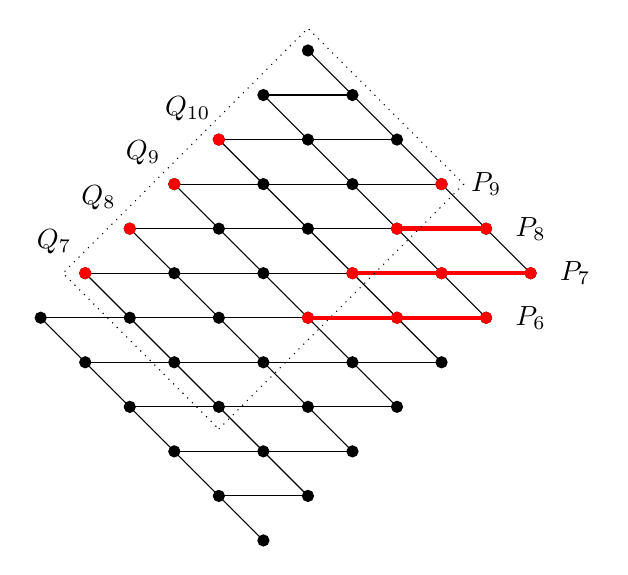
\begin{tikzpicture}[scale = .8, rotate = 135]
%EDGES
\tikzset{v/.style={circle, draw, inner sep=0pt, minimum width=4pt}}
\foreach \i in {1,...,6}
    \foreach \j in {1,...,7}
        \node[v,fill=black] at (\i,-\j){};
\foreach \i in {1,...,5}
    \foreach \j in {1,...,7}
        \draw (\i,-\j)--(\i+1,-\j);
\foreach \i in {1,...,5}
    \foreach \j in {2,...,7}
        \draw (\i,-\j)--(\i+1,-\j+1);
\foreach \i/\j in {3/7,3/6,3/5,3/4,2/7,2/6,2/5,1/7,1/6,6/2,6/3,6/4,6/5}
    \node[v,draw=red,fill=red] at (\i,-\j){};
\draw[ultra thick,red] (2,-7)--(3,-6) (1,-7)--(3,-5) (1,-6)--(3,-4);
\draw[dotted] (2.75,-1.75) rectangle (6.25,-7.25);
\node at (.5,-6.5) {$P_6$};
\node at (.5,-7.5) {$P_7$};
\node at (1.5,-7.5) {$P_8$};
\node at (2.5,-7.5) {$P_9$};
\node at (6.7,-2) {$Q_7$};
\node at (6.7,-3) {$Q_8$};
\node at (6.7,-4) {$Q_9$};
\node at (6.7,-5) {$Q_{10}$};
% \draw [red,very thick] (0,0)--(1,0);
% \draw [very thick] (1,0)--(2,0);
% \draw [red,very thick] (0,-1)--(1,-1);
% \draw [very thick] (1,-1)--(2,-1);
% \draw [red, very thick] (0,-2)--(1,-2);
% \draw [very thick] (1,-2)--(2,-2);

% \draw [very thick] (0,-1)--(1,0);
% \draw [very thick] (0,-2)--(1,-1);
% \draw [red, very thick] (1,-1)--(2,0);
% \draw [red, very thick] (1,-2)--(2,-1);

% %NODES
% \draw [red, fill=red] (0,0) circle [radius=0.08cm];
% \draw [red, fill=red] (1,0) circle [radius=0.08cm];
% \draw [red, fill=red] (2,0) circle [radius=0.08cm];

% \draw [red, fill=red] (0,-1) circle [radius=0.08cm];
% \draw [red, fill=red] (1,-1) circle [radius=0.08cm];
% \draw [red, fill=red] (2,-1) circle [radius=0.08cm];

% \draw [red, fill=red] (0,-2) circle [radius=0.08cm];
% \draw [red, fill=red] (1,-2) circle [radius=0.08cm];
% \draw [fill=black] (2,-2) circle [radius=0.08cm];

% \begin{scriptsize}
% \node at (-0.2,-0.2) {$P_0$};
% \node at (-0.2,-1.2) {$P_1$};
% \node at (-0.2,-2.2) {$P_2$};

% \node at (1.2,0.2) {$Q_1$};
% \node at (2.2,0.2) {$Q_2$};
% \node at (2.2,-0.8) {$Q_3$};

% \node at (0.35,-0.23) {$x_{0,0}^{-1}$};
% \node at (1.35,-0.23) {$x_{1,0}^{-1}$};

% \node at (0.35,-1.23) {$x_{0,1}^{-1}$};
% \node at (1.35,-1.23) {$x_{1,1}^{-1}$};

% \node at (0.35,-2.23) {$x_{0,2}^{-1}$};
% \node at (1.35,-2.23) {$x_{1,2}^{-1}$};
% \end{scriptsize}
\end{tikzpicture}
\caption{Illustration of $\mathcal G_R$ and $\mathcal G_I$ (dotted) for $R = [5] \times [7]$ and $I = [3,5] \times [2,7]$ with $k=2$ as in Corollary~\ref{pathsinideal} (note $j_2=s$ and $i_2=r$). Nonintersecting paths from $\{P_6, \dots P_9\}$ to $\{Q_7, \dots, Q_{10}\}$ in $\mathcal G_R$ must contain the horizontal steps shown.}
\label{fig:pathsinorderideal}
\end{figure}

In particular, note that the conditions of Corollary~\ref{pathsinideal} hold whenever $I$ is an order ideal (when $i_1=j_1=1$) or order filter (when $i_2=r$ and $j_2=s$) of $R$.


\subsection{Birational rowmotion formula}

Using the relation between the octahedron recurrence and toggles, we will prove the following birational rowmotion formula.

\begin{Th}
\label{birationalrowmotionformula}
Let $R = [r] \times [s]$, $x \in \mathbb{R}_{>0}^{R}$, and $y = \phi^{-1}(x)$. %Label the edges of $(i,j) \to (i+1,j)$ in $\mathcal{G}_R$ with $x_{ij}^{-1}$ and all other edges in $\mathcal{G}_R$ with label 1. 
Fix $(i,j) \in R$.

%Label the edges of $\mathcal G_R$ with respect to $x$ as described above, and let $(i,j) \in R$.

%For $0 \leq u,v \leq r+s+1$ let $P_u = (\max(u-s,0), \min(u,s))$ and $Q_v = (\min(v,r), \max(v-r,0))$. Let $y \in \mathbb{R}_{>0}^{R}$ and let $x = \phi(y)$. Label $\mathcal{G}_R$ as above using the labelling $x$ of the rectangle. Let $W_a^b(c)$ denote the sum of the weights of all non-intersecting lattice paths from $(P_a,...,P_{a+c-1})$ to $(Q_b,...,Q_{b+c-1})$. If $0 \leq k \leq r+s+1$ and $i+j \leq r+s-k$, then

\begin{enumerate}[(a)]
\item If $0 \leq k \leq r+s-i-j$, then
\[\rho^{-k}(y)_{ij} = \frac{W_{k+2,i+k+1}^{(j-1)}}{W_{k+1,i+k+1}^{(j)}}.\]
\item For all $k \in \mathbb{Z}$,
\[\rho^{k}(y)_{ij} = \frac{1}{\rho^{k-i-j+1}(y)_{r+1-i,s+1-j}}.\]
In particular, if $0 < k < i+j$, then the right hand side can be computed using part (a).
%In particular, if $0 \leq k \leq r+s+1$ and $i+j > r+s-k$, then $\rho^{k-i-j}(y)_{r-i,s-j}$ can be calculated from part (a).
\item For all $k \in \mathbb Z$, $\rho^{k+r+s}(y) = \rho^k(y)$. In other words, the action of rowmotion on $R$ has order $r+s$.
\end{enumerate}
\end{Th}

%In the array, each labelling is of the form $W_a^b(c)$ and the value of $\rho^{-k}(y)_{i,j}$ is stored in pairs of labellings. To obtain $y_{i,j}$ from $M$, we claim that $y_{i,j} = \frac{M_{2,2i+2,j}}{M_{0,2i+2,j+1}}$, and that applying inverse rowmotion yields the array shifted by $(2,2,0)$. Note that in the figure below, shifting the array of edges by $(2,2,0)$ causes part of the edge corresponding to the label of $(r,s)$ to exit the array, and so Part A cannot compute this coordinate. Indeed, after each application of $\rho^{-k}$ and each shift by $(2,2,0)$, we lose the ability to compute the value at yet another rank.

%Label the rectangle $R = [0,r] \times [0,s]$ as below (this is the labeling obtained after applying the transfer map).

% \begin{figure}
% \begin{tikzpicture}[scale = 1.3, rotate = 135]
% \transparent{0.0};
% \draw [blue] (-0.7,0.2)--(0.5,-1);
% \draw [blue] (0.5,-1)--(-0.5,-2);
% \transparent{1.0};

% %EDGES
% \draw (0,0)--(1,0);
% \draw (0,-1)--(1,-1);
% \draw (0,-2)--(1,-2);

% \draw (0,0)--(0,-2);
% \draw (1,0)--(1,-2);

% %NODES
% \draw [fill=black] (0,0) circle [radius=0.08cm];
% \draw [fill=black] (1,0) circle [radius=0.08cm];

% \draw [fill=black] (0,-1) circle [radius=0.08cm];
% \draw [fill=black] (1,-1) circle [radius=0.08cm];

% \draw [fill=black] (0,-2) circle [radius=0.08cm];
% \draw [fill=black] (1,-2) circle [radius=0.08cm];

% \begin{small}
% \node at (-0.2,-0.2) {$a$};
% \node at (-0.2,-1.2) {$c$};
% \node at (-0.2,-2.2) {$e$};

% \node at (0.8,-0.2) {$b$};
% \node at (0.8,-1.2) {$d$};
% \node at (0.8,-2.2) {$f$};
% \end{small}

% \end{tikzpicture}
% \caption{}
% \label{fig:rectangle}
% \end{figure}

\begin{figure}
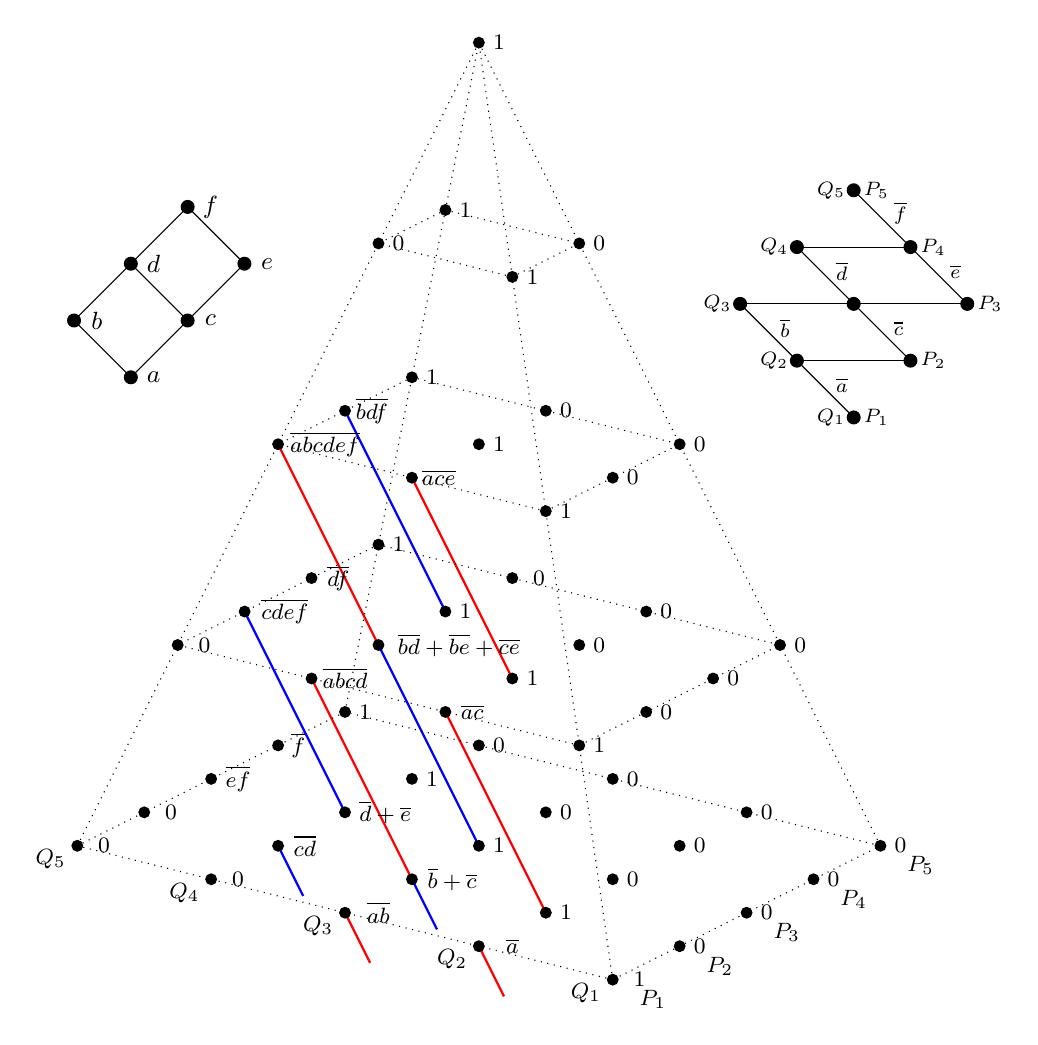
\begin{tikzpicture}[scale = 0.85]

%R
\begin{scope}[scale=1.2,shift={(-6,7.5)},rotate=135]
%EDGES
\draw (0,0)--(1,0);
\draw (0,-1)--(1,-1);
\draw (0,-2)--(1,-2);

\draw (0,0)--(0,-2);
\draw (1,0)--(1,-2);

%NODES
\draw [fill=black] (0,0) circle [radius=0.08cm];
\draw [fill=black] (1,0) circle [radius=0.08cm];

\draw [fill=black] (0,-1) circle [radius=0.08cm];
\draw [fill=black] (1,-1) circle [radius=0.08cm];

\draw [fill=black] (0,-2) circle [radius=0.08cm];
\draw [fill=black] (1,-2) circle [radius=0.08cm];

\begin{small}
\node at (-0.2,-0.2) {$a$};
\node at (-0.2,-1.2) {$c$};
\node at (-0.2,-2.2) {$e$};

\node at (0.8,-0.2) {$b$};
\node at (0.8,-1.2) {$d$};
\node at (0.8,-2.2) {$f$};
\end{small}
\end{scope}

\begin{scope}[scale = 1.2, shift={(3,7.0)}, rotate = 135]
%EDGES
\draw (0,0)--(1,0);
\draw (1,0)--(2,0);
\draw (0,-1)--(2,-1);
\draw (0,-2)--(1,-2);
\draw (1,-2)--(2,-2);

\draw (0,-1)--(1,0);
\draw (0,-2)--(2,0);
\draw (1,-2)--(2,-1);

%NODES
\draw [fill=black] (0,0) circle [radius=0.08cm];
\draw [fill=black] (1,0) circle [radius=0.08cm];
\draw [fill=black] (2,0) circle [radius=0.08cm];

\draw [fill=black] (0,-1) circle [radius=0.08cm];
\draw [fill=black] (1,-1) circle [radius=0.08cm];
\draw [fill=black] (2,-1) circle [radius=0.08cm];

\draw [fill=black] (0,-2) circle [radius=0.08cm];
\draw [fill=black] (1,-2) circle [radius=0.08cm];
\draw [fill=black] (2,-2) circle [radius=0.08cm];

\begin{scriptsize}
\node at (-0.2,-0.2) {$P_1$};
\node at (-0.2,-1.2) {$P_2$};
\node at (-0.2,-2.2) {$P_3$};
\node at (0.8,-2.2) {$P_4$};
\node at (1.8,-2.2) {$P_5$};

\node at (0.2,0.2) {$Q_1$};
\node at (1.2,0.2) {$Q_2$};
\node at (2.2,0.2) {$Q_3$};
\node at (2.2,-0.8) {$Q_4$};
\node at (2.2,-1.8) {$Q_5$};

\node at (0.39,-0.18) {$\overline{a}$};
\node at (1.39,-0.18) {$\overline{b}$};

\node at (0.39,-1.18) {$\overline{c}$};
\node at (1.39,-1.18) {$\overline{d}$};

\node at (0.39,-2.18) {$\overline{e}$};
\node at (1.39,-2.21) {$\overline{f}$};
\end{scriptsize}
\end{scope}


\draw [red,thick] (-1.625,-0.25)--(-2,0.5);
\draw [red,thick] (-3.625,0.25)--(-4,1);

\draw [red,thick] (-1,1)--(-2.5,4);
\draw [red,thick] (-3,1.5)--(-4.5,4.5);

\draw [red,thick] (-1.5,4.5)--(-3,7.5);
\draw [red,thick] (-3.5,5)--(-5,8);

\draw [blue,thick] (-2.625,0.75)--(-3,1.5);
\draw [blue,thick] (-4.625,1.25)--(-5,2);

\draw [blue,thick] (-2,2)--(-3.5,5);
\draw [blue,thick] (-4,2.5)--(-5.5,5.5);

\draw [blue,thick] (-2.5,5.5)--(-4,8.5);
%\draw [blue,thick] (-4.5,6)--(-6,9);

%LAYER 1
\draw [fill=black] (0,0) circle [radius=0.08cm];
\draw [fill=black] (-2,0.5) circle [radius=0.08cm];
\draw [fill=black] (-4,1) circle [radius=0.08cm];
\draw [fill=black] (-6,1.5) circle [radius=0.08cm];
\draw [fill=black] (-8,2) circle [radius=0.08cm];

\draw [fill=black] (1,0.5) circle [radius=0.08cm];
\draw [fill=black] (-1,1) circle [radius=0.08cm];
\draw [fill=black] (-3,1.5) circle [radius=0.08cm];
\draw [fill=black] (-5,2) circle [radius=0.08cm];
\draw [fill=black] (-7,2.5) circle [radius=0.08cm];

\draw [fill=black] (2,1) circle [radius=0.08cm];
\draw [fill=black] (0,1.5) circle [radius=0.08cm];
\draw [fill=black] (-2,2) circle [radius=0.08cm];
\draw [fill=black] (-4,2.5) circle [radius=0.08cm];
\draw [fill=black] (-6,3) circle [radius=0.08cm];

\draw [fill=black] (3,1.5) circle [radius=0.08cm];
\draw [fill=black] (1,2) circle [radius=0.08cm];
\draw [fill=black] (-1,2.5) circle [radius=0.08cm];
\draw [fill=black] (-3,3) circle [radius=0.08cm];
\draw [fill=black] (-5,3.5) circle [radius=0.08cm];

\draw [fill=black] (4,2) circle [radius=0.08cm];
\draw [fill=black] (2,2.5) circle [radius=0.08cm];
\draw [fill=black] (0,3) circle [radius=0.08cm];
\draw [fill=black] (-2,3.5) circle [radius=0.08cm];
\draw [fill=black] (-4,4) circle [radius=0.08cm];

%LAYER 2
\draw [fill=black] (-0.5,3.5) circle [radius=0.08cm];
\draw [fill=black] (-2.5,4) circle [radius=0.08cm];
\draw [fill=black] (-4.5,4.5) circle [radius=0.08cm];
\draw [fill=black] (-6.5,5) circle [radius=0.08cm];

\draw [fill=black] (0.5,4) circle [radius=0.08cm];
\draw [fill=black] (-1.5,4.5) circle [radius=0.08cm];
\draw [fill=black] (-3.5,5) circle [radius=0.08cm];
\draw [fill=black] (-5.5,5.5) circle [radius=0.08cm];

\draw [fill=black] (1.5,4.5) circle [radius=0.08cm];
\draw [fill=black] (-0.5,5) circle [radius=0.08cm];
\draw [fill=black] (-2.5,5.5) circle [radius=0.08cm];
\draw [fill=black] (-4.5,6) circle [radius=0.08cm];

\draw [fill=black] (2.5,5) circle [radius=0.08cm];
\draw [fill=black] (0.5,5.5) circle [radius=0.08cm];
\draw [fill=black] (-1.5,6) circle [radius=0.08cm];
\draw [fill=black] (-3.5,6.5) circle [radius=0.08cm];

%LAYER 3
\draw [fill=black] (-1,7) circle [radius=0.08cm];
\draw [fill=black] (-3,7.5) circle [radius=0.08cm];
\draw [fill=black] (-5,8) circle [radius=0.08cm];

\draw [fill=black] (0,7.5) circle [radius=0.08cm];
\draw [fill=black] (-2,8) circle [radius=0.08cm];
\draw [fill=black] (-4,8.5) circle [radius=0.08cm];

\draw [fill=black] (1,8) circle [radius=0.08cm];
\draw [fill=black] (-1,8.5) circle [radius=0.08cm];
\draw [fill=black] (-3,9) circle [radius=0.08cm];

%LAYER 4
\draw [fill=black] (-1.5,10.5) circle [radius=0.08cm];
\draw [fill=black] (-3.5,11) circle [radius=0.08cm];

\draw [fill=black] (-2.5,11.5) circle [radius=0.08cm];
\draw [fill=black] (-0.5,11) circle [radius=0.08cm];

%LAYER 5
\draw [fill=black] (-2,14) circle [radius=0.08cm];

%DOTTED LINES
\draw [dotted] (0,0)--(-8,2)--(-4,4)--(4,2)--cycle;
\draw [dotted] (-0.5,3.5)--(-6.5,5)--(-3.5,6.5)--(2.5,5)--cycle;
\draw [dotted] (-1,7)--(-5,8)--(-3,9)--(1,8)--cycle;
\draw [dotted] (-1.5,10.5)--(-3.5,11)--(-2.5,11.5)--(-0.5,11)--cycle;


%\draw [dotted] (0,0)--(-1,7);
%\draw [dotted] (-8,2)--(-5,8);
%\draw [dotted] (-4,4)--(-3,9);
%\draw [dotted] (4,2)--(1,8);

\draw [dotted] (0,0)--(-2,14);
\draw [dotted] (-8,2)--(-2,14);
\draw [dotted] (-4,4)--(-2,14);
\draw [dotted] (4,2)--(-2,14);

\begin{footnotesize}
%LAYER 1
\node at (0.4,0) {$1$};
\node at (-1.5,0.5) {$\overline{a}$};
\node at (-3.5,1) {$\overline{ab}$};
\node at (-5.6,1.5) {$0$};
\node at (-7.6,2) {$0$};

\node at (1.3,0.5) {$0$};
\node at (-0.7,1) {$1$};
\node at (-2.4,1.5) {$\overline{b} + \overline{c}$};
\node at (-4.6,2) {$\overline{cd}$};
\node at (-6.6,2.5) {$0$};

\node at (2.3,1) {$0$};
\node at (0.3,1.5) {$0$};
\node at (-1.7,2) {$1$};
\node at (-3.4,2.5) {$\overline{d} + \overline{e}$};
\node at (-5.6,3) {$\overline{ef}$};

\node at (3.3,1.5) {$0$};
\node at (1.3,2) {$0$};
\node at (-0.7,2.5) {$0$};
\node at (-2.7,3) {$1$};
\node at (-4.7,3.5) {$\overline{f}$};

\node at (4.3,2) {$0$};
\node at (2.3,2.5) {$0$};
\node at (0.3,3) {$0$};
\node at (-1.7,3.5) {$0$};
\node at (-3.7,4) {$1$};

%LAYER 2
\node at (-0.2,3.5) {$1$};
\node at (-2.1,4) {$\overline{ac}$};
\node at (-4.0,4.5) {$\overline{abcd}$};
\node at (-6.1,5) {$0$};

\node at (0.8,4) {$0$};
\node at (-1.2,4.5) {$1$};
\node at (-2.3,5) {$\overline{bd} + \overline{be} + \overline{ce}$};
\node at (-4.9,5.5) {$\overline{cdef}$};

\node at (1.8,4.5) {$0$};
\node at (-0.2,5) {$0$};
\node at (-2.2,5.5) {$1$};
\node at (-4.1,6) {$\overline{df}$};

\node at (2.8,5) {$0$};
\node at (0.8,5.5) {$0$};
\node at (-1.1,6) {$0$};
\node at (-3.2,6.5) {$1$};

%LAYER 3
\node at (-0.7,7) {$1$};
\node at (-2.6,7.5) {$\overline{ace}$};
\node at (-4.3,8) {$\overline{abcdef}$};

\node at (0.3,7.5) {$0$};
\node at (-1.7,8) {$1$};
\node at (-3.6,8.5) {$\overline{bdf}$};

\node at (1.3,8) {$0$};
\node at (-0.7,8.5) {$0$};
\node at (-2.7,9) {$1$};

%LAYER 4
\node at (-1.2,10.5) {$1$};
\node at (-3.2,11) {$0$};

\node at (-0.2,11) {$0$};
\node at (-2.2,11.5) {$1$};

%LAYER 5
\node at (-1.7,14) {$1$};


%P's and Q's
\node at (-0.4,-0.2) {$Q_1$};
\node at (-2.4,0.3) {$Q_2$};
\node at (-4.4,0.8) {$Q_3$};
\node at (-6.4,1.3) {$Q_4$};
\node at (-8.4,1.8) {$Q_5$};

\node at (0.6,-0.3) {$P_1$};
\node at (1.6,0.2) {$P_2$};
\node at (2.6,0.7) {$P_3$};
\node at (3.6,1.2) {$P_4$};
\node at (4.6,1.7) {$P_5$};
\end{footnotesize}
\end{tikzpicture}
\caption{$R=[2] \times [3]$, $\mathcal G_R$, and the corresponding array $W=W_{ij}^{(k)}$ for $1 \leq k \leq 5$, where $\overline{a}$ denotes $a^{-1}$ for readability. (All entries at height $0$ equal $1$, and all other entries not shown are $0$.) Red and blue lines indicate quotients used to compute $\rho^0(y)=y=\phi^{-1}(x)$ and $\rho^{-1}(y)$ (apart from the topmost label), respectively.}
\label{fig:array}
\end{figure}


Theorem~\ref{birationalrowmotionformula} can be used to find an explicit formula for the entries of any power of $\rho$ applied to $y$. (Using parts (a) and (b) one can compute $\rho^{k}(y)_{ij}$ whenever $i+j-r-s \leq k < i+j$, and part (c) can be used to bring $k$ into this range.) While the birational rowmotion formulas given in \cite{musikerroby} are stated in terms of complements of paths in $R$, the formulation given here can be seen to be equivalent using Corollary~\ref{pathsinideal}.

Geometrically, Theorem~\ref{birationalrowmotionformula}(a) states that one can find the values of $\rho^{-k}(y)_{ij}$ as quotients of nearby entries inside the array $W$, and increasing the value of $k$ corresponds to a translation in the direction $(1,1,0)$ as long as these entries remain inside the defined pyramidal region of $W$. Upon passing outside this region, one needs to use part (b) to relocate inside the pyramid to the entries corresponding to the antipodal point of $R$. See Figure~\ref{fig:array}.

\begin{Ex}
Let $R = [2] \times [3]$. Let $x$ be the labeling of $R$ as in Figure~\ref{fig:array} with the array $(W_{ij}^{(k)})$ as previously described. When $(i,j)=(2,2)$, Theorem \ref{birationalrowmotionformula}(a) gives
%We construct the matrix $A$ from the induced labeling on $\mathcal{G}_R$ such that $a_{ij}$ is the sum of the weights of all paths from $P_{i}$ to $Q_{j}$. Using the Dodgson condensation formula, we construct the array in Figure \ref{fig:array}. The missing labels in the pyramid form the identity matrix at each height. We will use the array to compute the powers of rowmotion on $R = [0,1] \times [0,2]$ at $(1,1)$.
\begin{align*}
    \rho^{0}(y)_{22} &= \frac{W_{23}^{(1)}}{W_{13}^{(2)}} =  \frac{b^{-1} + c^{-1}}{(abcd)^{-1}} = acd + abd,\\
    \rho^{-1}(y)_{22} &= \frac{W_{34}^{(1)}}{W_{24}^{(2)}} = \frac{d^{-1} + e^{-1}}{(cdef)^{-1}} = cef + cdf.
\end{align*}

To compute $\rho^{-2}(y)_{22}$, $r+s-i-j = 1 < 2$, so part (a) does not apply. Instead, we apply parts (c) and (b) first to obtain
\begin{align*}
    \rho^{-2}(y)_{22} &= \rho^{3}(y)_{22} = \frac{1}{\rho^{0}(y)_{12}} = \frac{W_{12}^{(2)}}{W_{22}^{(1)}}\\
    &= (ac)^{-1}, \\
    \rho^{-3}(y)_{22} &= \rho^2(y)_{22} = \frac{1}{\rho^{-1}(y)_{12}} = \frac{W_{23}^{(2)}}{W_{33}^{(1)}} \\&= (bd)^{-1}+(be)^{-1}+(ce)^{-1},\\
    \rho^{-4}(y)_{22} &= \rho(y)_{22} = \frac{1}{\rho^{-2}(y)_{12}} =
    \frac{W_{34}^{(2)}}{W_{44}^{(1)}} \\&= (df)^{-1}.
\end{align*}
\end{Ex}

We will prove each part of Theorem~\ref{birationalrowmotionformula} separately. Part (a) follows primarily from Lemma~\ref{lemma:arraytoggle}, though some care is needed along the boundary of $R$.


\begin{proof}[Proof of Theorem~\ref{birationalrowmotionformula}(a)]
Let $z_{ij}^{(k)} = \frac{W_{k+2,i+k+1}^{(j-1)}}{W_{k+1,i+k+1}^{(j)}}$, which we wish to equal $\rho^{-k}(y)_{ij}$ for $0 \leq k \leq r+s-i-j$. We proceed by induction on $k$. When $k = 0$, $\rho^0(y)_{ij} = y_{ij} = \phi^{-1}(x)_{ij}$ is the total weight of all maximal chains in $[i] \times [j]$ (with respect to the labeling $x$). By Corollary~\ref{pathsinideal}(b), this is $\frac{W_{2,i+1}^{(j-1)}}{W_{1,i+1}^{(j)}} = z_{ij}^{(0)}$, as desired.

% consider the denominator $W_{0,i+1}^{(j+1)}$. This is the total weight of systems of nonintersecting paths in $\mathcal{G}_R$ from $P_0,\dots,P_j$ to $Q_{i+1},\dots,Q_{i+j+1}$. By Corollary~\ref{pathsinideal} this weight is $\prod\limits_{p \in \Lambda_{ij}} x_p^{-1}$.

% %Note that in any collection of nonintersecting lattice paths, the path starting at $P_\ell$ must travel to $Q_{i+\ell+1}$. Since $i \leq r$, there is a unique path from $P_0 = (0,0)$ to $Q_{i+1} = (i+1,0)$ given by traversing diagonal edges. This forces the path from $P_1$ to $Q_{i+2}$ to traverse the first $i$ diagonal edges available to it (See the figure below). After this, the only path available to the destination is horizontal edges. Continuing to construct paths in this fashion gives a unique set of nonintersecting lattice paths, which has weight $\prod\limits_{p \in \Lambda_{i,j}} x_p^{-1}$.

% The numerator $W_{1,i+1}^{(j)}$ is the weight of nonintersecting paths in $\mathcal{G}_R$ from $P_1,\dots,P_j$ to $Q_{i+1},\dots, Q_{i+j}$. By Corollary \ref{pathsinideal} the weight of each system of paths is the inverse weight of the complement of a path from $(0,0)$ to $(i,j)$ in $R$. Dividing by $\prod\limits_{p \in \Lambda_{i,j}} x_p^{-1}$ gives the sum of weights of all nonintersecting lattice paths from $(0,0)$ to $(i,j)$ in $R$. This value is $y_{i,j} = \phi^{-1}(x)_{i,j}$ as desired.

%Paths must end at the $Q_\ell$, which must end in horizontal steps after leaving the last edge in $\Lambda_{i,j}$. Letting $Q_\ell' = (i+1,\ell)$, the set of nonintersecting lattice paths from $P$ to $Q'$ are in bijection with lattice paths from $(0,0)$ to $(i,j)$ in $R$. So the weights of nonintersecting lattice paths from $P$ to $Q$ are complements of paths from $(0,0)$ to $(i,j)$ in $R$. Dividing by $\prod\limits_{p \in \Lambda_{i,j}} x_p^{-1}$ gives the sum of weights of all nonintersecting lattice paths from $(0,0)$ to $(i,j)$ as desired. 

For the inductive step, assume $k > 0$ and suppose that the claim is true for $\rho^{-k+1}(y)$ as well as for $\rho^{-k}(y)_{i'j'}$ when $(i',j') < (i,j)$. The value of $\rho^{-k}(y)$ is obtained by applying toggles from bottom to top on $\rho^{-k+1}(y)$, so the toggle at $(i,j)$ gives
\[\rho^{-k}(y)_{ij} = \left(\sum_{(i',j')\lessdot (i,j)} \rho^{-k}(y)_{i'j'}\right)\left(\;\;\;\sideset{}{^{\parallelsum}}\sum_{(i',j') \gtrdot (i,j)}\rho^{-k+1}(y)_{i'j'}\right) \cdot \frac{1}{\rho^{-k+1}(y)_{ij}}, \tag{$*$} \label{eq:toggle}\]
where an empty sum is replaced with $1$. 

We claim that we can replace the first sum in \eqref{eq:toggle} with $z_{i,j-1}^{(k)}+z_{i-1,j}^{(k)}$. If $i > 1$ and $j > 1$, then this is immediate by induction. Otherwise note that
\[
    z_{i0}^{(k)} = \frac{W_{k+2,i+k+1}^{(-1)}}{W_{k+1,i+k+1}^{(0)}} = \frac01= 0,\qquad
    z_{0j}^{(k)} = \frac{W_{k+2,k+1}^{(j-1)}}{W_{k+1,k+1}^{(j)}} = \frac{\delta_{j1}}{1} = \delta_{j1}
\]
by Proposition~\ref{prop:wproperties}(a) and (b).
Thus if exactly one of $i$ and $j$ is $1$, then one of $z_{i,j-1}^{(k)}$ and $z_{i-1,j}^{(k)}$ equals $0$ while the other is the only term in the first sum in \eqref{eq:toggle} by induction. If instead $i=j=1$, then the empty sum in \eqref{eq:toggle} is replaced with $1=0 + \delta_{11} = z_{10}^{(k)} + z_{01}^{(k)}$ as needed.

Similarly, we claim that we can replace the second (parallel) sum in \eqref{eq:toggle} with either $z_{i,j+1}^{(k-1)} \parallelsum z_{i+1,j}^{(k-1)}$, or just one of these terms if the other is undefined. If $i < r$ and $j < s$, then this is again immediate by induction (since the inequality $k-1 \leq r+s-(i+j+1)$ holds). If $i=r$ and $j < s$, then $z_{r+1,j}^{(k-1)}$ is undefined since $W_{k,r+k+1}^{(j)}=0$ by Proposition~\ref{prop:wproperties}(a), so we are left with $z_{r,j+1}^{(k-1)} = \rho^{-k+1}(y)_{r,j+1}$ by induction. If instead $i < r$ and $j=s$, then $z_{i,s+1}^{(k-1)}$ is undefined since $W_{k,i+k}^{(s+1)} = 0$ by Proposition~\ref{prop:wproperties}(c), which leaves just $z_{i+1,s}^{(k-1)} = \rho^{-k+1}(y)_{i+1,s}$ by induction. Finally, $i=r$ and $j=s$ cannot both occur since $0 < k \leq r+s-i-j$.

The final factor in \eqref{eq:toggle} is equal to $\frac{1}{z^{(k-1)}_{ij}}$ by induction. The result then follows by comparing \eqref{eq:toggle} to Lemma~\ref{lemma:arraytoggle}, using Remark~\ref{rem:arraytoggle} when needed.
%
%
% determined by applying the toggle $t_{ij}$ to the following labeling (where some elements may be missing if $(i,j)$ lies on the outer boundary of $R$):
% \[\begin{tikzpicture}
% \node(1)[w,label=below left:{$\rho^{-k}(y)_{i,j-1}$}] at (-1,-1){};
% \node(2)[w,label=below right:{$\rho^{-k}(y)_{i-1,j}$}] at (1,-1){};
% \node(3)[w,label=right:{$\rho^{-k}(y)_{ij}$}] at (0,0){};
% \node(4)[w,label=above left:{$\rho^{-k+1}(y)_{i+1,j}$}] at (-1,1){};
% \node(5)[w,label=above right:{$\rho^{-k+1}(y)_{i,j+1}$}] at (1,1){};
% \draw (1)--(3)--(2) (4)--(3)--(5);
% \end{tikzpicture}
% \]
%
% If $(i,j)$ covers 2 elements and is covered by 2 elements and if $i+j \leq r+s-k$, then we have
%
% \begin{align*}
%     &\rho^{-k+1}(y)_{i+1,j} = \frac{M_{2k,2i+2k+2,j}}{M_{2k-2,2i+2k+2,j+1}}& & \rho^{-k+1}(y)_{i,j+1} = \frac{M_{2k,2i+2k,j+1}}{M_{2k-2,2i+2k,j+2}}\\
%     & &\rho^{-k+1}(y)_{i,j} = \frac{M_{2k,2i+2k,j}}{M_{2k-2,2i+2k,j+1}} & \\
%     &\rho^{-k}(y)_{i,j-1} = \frac{M_{2k+2,2i+2k+2,j-1}}{M_{2k,2i+2k+2,j}}& & \rho^{-k}(y)_{i-1,j} = \frac{M_{2k+2,2i+2k,j}}{M_{2k,2i+2k,j+1}} \\
% \end{align*}
% Note that here the inequality condition is required to use the array to compute $\rho^{-k+1}(y)_{i+1,j}$ and $\rho^{-k+1}(y)_{i,j+1}$ with the array. Shifting the array by the vector $(2-2k,2-2k,0)$ yields:
%
% \begin{align*}
%     &z_{i+1,j} = \frac{M_{2,2i+4,j}}{M_{0,2i+4,j+1}}& & z_{i,j+1} = \frac{M_{2,2i+2,j+1}}{M_{0,2i+2,j+2}}\\
%     & &z_{i,j} = \frac{M_{2,2i+2,j}}{M_{0,2i+2,j+1}} & \\
%     &z_{i,j-1} = \frac{M_{4,2i+4,j-1}}{M_{2,2i+4,j}}& & z_{i-1,j} = \frac{M_{4,2i+2,j}}{M_{2,2i+2,j+1}} \\
% \end{align*}
% Thus by Lemma \ref{lemma:arraytoggle},
%
% \[\frac{M_{2k+2,2i+2k+2,j}}{M_{2k,2i+2k+2,j+1}} = t_{i,j}\left(\rho^{-k+1}(y)\right)_{i,j} = \rho^{-k}(y)_{i,j}\]
% %Note that in Lemma \ref{lemma:arraytoggle} we showed that this toggle did not require all of these elements covering and covered by $(i,j)$ to exist; we only need one element covering $(i,j)$ to be computable via the induction step. Consequently Part A can be used to compute $\rho^{-k}(y)_{i,j}$ if and only if $i+j \leq r+s-k$.
%
% If $(i,j)$ lies on the boundary of $R$, we claim that the octahedron recurrence still simulates toggles. Label the unlabeled elements in the lattice $x \equiv y \equiv 0$ mod $2$ by $0$. If $(i,j)=(0,0)$, let
% \begin{align*}
%     z_{0,-1} = \frac{f(4,4,-1)}{f(2,4,0)} = 0& &z_{-1,0} = \frac{f(4,2,0)}{f(2,2,1)} = 1
% \end{align*}
% which are informally the ratios of the edges of the octahedron which correspond to the nonexistent elements covered by $(0,0)$. We subsitute these into the toggle expression that we computed from the octahedron recurrence in Lemma \ref{lemma:arraytoggle}:
%
% \begin{align*}
%     &\left(z_{0,-1} + z_{-1,0}\right)\left(\rho^{-k+1}(y)_{1,0} \parallelsum \rho^{-k+1}(y)_{0,1}\right)\frac{1}{\rho^{-k+1}(y)_{0,0}} \\
%     &= \left(\rho^{-k+1}(y)_{1,0} \parallelsum \rho^{-k+1}(y)_{0,1}\right)\frac{1}{\rho^{-k+1}(y)_{0,0}} \\
%     &= \rho^{-k}(y)_{0,0}
% \end{align*}
%
% The case of join irreducibles is similar. Now consider the case of $(r,j)$ where $r+j \leq r+s-k$, so that $\rho^{-k+1}(y)_{r,j+1}$ is computable by induction. The edge corresponding to the nonexistent element $(r+1,j)$ exits the array from above. Let $\frac{1}{z_{r+1,j}} = 0$. From the parallel sum in the toggle relation yielded by the octahedron recurrence, we have
%
% \[\frac{1}{ \frac{1}{\rho^{-k+1}(y)_{r,j+1}} + \frac{1}{z_{r+1,j}}} = \rho^{-k+1}(y)_{r,j+1}\]
% Substituting this into the toggle expression yields the toggle at $(r,j)$.
%
% Finally, if $i+j = r+s-k+1$, then by induction $\rho^{-k+1}$ is not computable via Part A of the rowmotion formula at any element covering $(i,j)$. In fact, the associated edges of the octahedron exit the top of the array. In this case, the parallel sum in the toggle relation yields division by 0. Hence Part A cannot compute $\rho^{-k}(y)_{i,j}$.
\end{proof}

Next we prove part (b). In some sense, this reflects two symmetries: toggling is respected by dualizing a poset and inverting each label, and the octahedron recurrence is respected by reflecting over the plane perpendicular to the main diagonal.

\begin{proof}[Proof of Theorem~\ref{birationalrowmotionformula}(b)]
Note that if $0 < k < i+j$, then $0 \leq i+j-k-1 \leq r+s-(r+1-i)-(s+1-j)$, so the right hand side of (b) will satisfy the condition of part (a), as claimed.

Via the change of coordinates $z = \rho^{k-1}(y)$, it suffices to prove the case when $k=1$. %, that is,
%\[\rho(y)_{i,j} = \frac{1}{\rho^{-i-j}(y)_{r-i,s-j}}.\]
By part (a),
\[\rho^{2-i-j}(y)_{r+1-i,s+1-j} = 
    \frac{W_{i+j,r+j}^{(s-j)}}{W_{i+j-1,r+j}^{(s-j+1)}}.\]
%The denominator is the sum of the weights of all nonintersecting lattice paths in $\mathcal{G}_R$ from $P_{i+j},\dots,P_{i+s}$ to $Q_{r+j+1},\dots,Q_{r+s+1}$. By Corollary \ref{pathsinideal} the weight of these paths is $\prod\limits_{z \in V_{i,j}} x_z^{-1}$. The numerator is the sum of the weights of all nonintersecting lattice paths in $\mathcal{G}_R$ from $P_{i+j+1},\dots, P_{i+s}$ to $Q_{r+j+1},\dots,Q_{r+s}$. 
%By Corollary~\ref{pathsinideal}, the weight of these paths is the sum of the inverse weights of complements of paths from $(i,j)$ to $(r,s)$ in $V_{i,j}$ (i.e. maximal chains). Let $\mathcal{P}$ denote paths in $V_{i,j}$ from $(i,j)$ to $(r,s)$ in $R$. Then
By Corollary~\ref{pathsinideal}, this is the total weight of all maximal chains in $[i,r] \times [j,s]$ in $R$ (with respect to the labeling $x$). Thus
%\[\rho^{-i-j}(y)_{r-i,s-j} = \frac{\sum\limits_{L \in \mathcal{P}} \prod\limits_{z \in V_{i,j} \setminus L} x_z^{-1}}{\prod\limits_{z \in V_{i,j}} x_z^{-1}} = \sum\limits_{L \in \mathcal{P}} \prod\limits_{z \in L} x_z = \left(\phi^*\right)^{-1}(x)_{i,j} = \frac{1}{\rho(y)_{i,j}}.\qedhere\]
\[\rho^{2-i-j}(y)_{r+1-i,s+1-j} = \left(\phi^*\right)^{-1}(x)_{ij} = \frac{1}{\rho(y)_{ij}}\]
by Lemma~\ref{lemma:dualtransfer}.
\end{proof}

%\begin{figure}
%\begin{tikzpicture}
%DIAGONAL EDGES
%\foreach \x in {0,...,3}{
%\draw (\x,\x)--(-2+\x,2+\x);
%}

%HORIZONTAL EDGES
%\draw (1,1)--(-1,1);
%\draw (2,2)--(-2,2);
%\draw (3,3)--(-1,3);
%\draw (2,4)--(-0,4);

%CIRCLES
%\draw [fill=black] (0,0) circle [radius=0.08cm];
%\draw [fill=black] (-1,1) circle [radius=0.08cm];
%\draw [red, fill=red] (-2,2) circle [radius=0.08cm];

%\draw [fill=black] (1,1) circle [radius=0.08cm];
%\draw [red, fill=red] (0,2) circle [radius=0.08cm];
%\draw [red, fill=red] (-1,3) circle [radius=0.08cm];

%\draw [red, fill=red] (2,2) circle [radius=0.08cm];
%\draw [red, fill=red] (1,3) circle [radius=0.08cm];
%\draw [red, fill=red] (0,4) circle [radius=0.08cm];

%\draw [red, fill=red] (3,3) circle [radius=0.08cm];
%\draw [red, fill=red] (2,4) circle [radius=0.08cm];
%\draw [fill=black] (1,5) circle [radius=0.08cm];

%LABELS
%\node at (2.4,2.3) {$P_2$};
%\node at (3.4,3.3) {$P_3$};
%\node at (2.4,4.3) {$P_4 = P'_4$};

%\node at (0.4,2.3) {$P'_2$};
%\node at (1.4,3.3) {$P'_3$};

%\node at (-1.6,2.3) {$Q_1$};
%\node at (-0.6,3.3) {$Q_2$};
%\node at (0.4,4.3) {$Q_3$};

%\draw [red, thick] (2,2)--(0,2);
%\draw [red, thick] (3,3)--(1,3);
%\end{tikzpicture}
%\caption{WHICH FIGURE IS IT}
%\end{figure}




%$i+j > r+s-k$, then 
%
%\[I+J = r-i+s-j \leq r-i+s-j+k = r+s-K\]
%
%\noindent where $I = r-i$, $J = s-j$, and $K = i+j-k$, so %$\rho^{k-i-j}(y)_{r-i,s-j}$ satisfies the condition in Part A of the birational rowmotion formula. \pushQED{\qed} \qedhere \popQED

Finally, we deduce part (c) from part (b).
%For completeness, we close this section with the computation appearing in \cite{musikerroby} of the period of birational rowmotion on the rectangle.
%
%\begin{Cor}
%Let $R = [0,r] \times [0,s]$. Then $\rho$ has period $r+s+2$.
%\end{Cor}

\begin{proof} [Proof of Theorem~\ref{birationalrowmotionformula}(c)]
Apply Theorem~\ref{birationalrowmotionformula}(b) twice:
\begin{align*}
    \rho^{k}(y)_{i,j} &= \left(\rho^{k-i-j+1}(y)_{r+1-i,s+1-j}\right)^{-1}\\ 
    &= \left[\left(\rho^{k-i-j+1-(r+1-i)-(s+1-j)+1}(y)_{i,j}\right)^{-1}\right]^{-1}\\
    & = \rho^{k-r-s}(y)_{i,j}.\qedhere
\end{align*}
\end{proof}

In the next two sections, we will show how to use the perspective relating rowmotion and the octahedron recurrence to prove various identities about rowmotion.
